\documentclass[10pt]{article}
\usepackage[margin=0.9in]{geometry}
\usepackage[T1]{fontenc}
\usepackage{lmodern,amsmath,amssymb,amsthm,booktabs,graphicx,hyperref}
\hypersetup{colorlinks=true,linkcolor=blue,citecolor=blue,urlcolor=blue}
\newtheorem{theorem}{Theorem}
\newtheorem{lemma}{Lemma}
\newtheorem{proposition}{Proposition}
\newcommand{\ind}{\mathbf{1}}
\newcommand{\TP}{\mathrm{TP}}
\newcommand{\TPR}{\mathrm{TPR}}
\newcommand{\FPR}{\mathrm{FPR}}
\newcommand{\Prec}{\mathrm{Prec}}
\newcommand{\NumSeries}{350}
\newcommand{\NumScores}{1050}
\newcommand{\MedianSpeedup}{2.06$\times$}
\newcommand{\MachineCPU}{Apple M1 Pro}
\newcommand{\PythonVersion}{3.12.4}

% The marked title, abstract, and body also generate the PVLDB counterpart.
\title{Support-Sensitive Exact VUS Evaluation}
\author{Youngmin Ko\\Independent Researcher\\Republic of Korea\\\texttt{rhdudals0505@naver.com}}
\date{21 October 2026\\\small Working manuscript; unsubmitted}
\begin{document}
\maketitle
\begin{abstract}
Volume Under the Surface (VUS) averages time-series anomaly-detection areas
over score thresholds and tolerance widths. We derive an exact scalar
evaluator for a pinned VUS definition. Score groups containing no position
in the maximum anomaly support contribute analytically integrable ROC
rectangles and zero PR area; retained events admit complete global ties.
Comparison-based preparation gives $O(n\log(Q+1)+(L+1)Q)$ time, where $Q$
is expanded support size and $L$ the largest width. Combining this reduction
with established radix ordering and linear interval geometry gives
$O(n+(L+1)Q)$ for finite binary64 inputs under the stated fixed-word and
unit-cost metric-arithmetic assumptions. Support restriction, cumulative
sums, and radix sorting are prior techniques; the VUS-specific reduction
eliminates inactive events while preserving their integral contributions.
An earlier comparison-based implementation evaluates both ROC and PR with
median speedups of $8.38\times$ and $4.55\times$ against released PR-only
fast-VUS on two CPUs. Against the fastest tested comparator, medians are
$2.04\times$ and $1.35\times$, with 209 and 574 of 2,100 cases slower or equal.
Optional width bounds reduce queries but can increase runtime; earlier
racing experiments increase aggregate cost. Exactness concerns the
all-threshold, all-width target, with floating-point agreement audited
numerically rather than bitwise.
\end{abstract}

% BEGIN SHARED BODY
\section{Introduction}
VUS averages range-aware ROC or precision--recall integrals across tolerance
widths, accounting for both overlap and whether an anomaly interval is hit
\cite{paparrizos2022,boniol2025}. Efficient evaluation matters: ESA-ADB explicitly
excluded VUS because of computational cost \cite{esa2024}. That observation
motivates speed improvements; it does not establish suitability for ESA-ADB's
other evaluation requirements.

The official optimized evaluator partitions static and dynamic labels and
restricts work to maximum-width anomaly support \cite{boniol2025}.
Klein's released fast-VUS further sorts support scores and uses cumulative
weighted sums \cite{klein2026}. These optimizations already avoid much repeated
work. We ask which threshold events can be eliminated altogether without
changing the scalar integrals. A score group containing no position in the
maximum anomaly support changes neither weighted positive mass nor existence
reward. Its ROC contribution can be integrated analytically, while its PR
contribution is zero. Removing such groups requires preserving the negative
rectangle before each retained event and admitting its complete global tie.

The resulting width sweep costs $O((L+1)Q)$ for expanded support size $Q$.
We give two preparation strategies: comparison-based support ranking with
global counts, and fixed-width radix ranking with a linear interval scan.
The latter yields $O(n+(L+1)Q)$ exhaustive evaluation for finite binary64
inputs under the assumptions of Proposition~\ref{prop:radix}. The contribution
is the VUS-specific event representation and its composition with established
ranking techniques, not a new sorting algorithm. Matching radix ranking,
interval geometry, and PR-only execution in dense controls is necessary to
assess the practical benefit of sparse event elimination.

The same event representation supports optional real-arithmetic width
enclosures and incremental model selection. Those extensions answer a
different question: whether avoiding width evaluations also reduces total
work. Earlier measurements show that query savings can be outweighed by
refinement and decision overhead. We retain these negative findings and the
full derivations in Appendices~\ref{sec:width} and~\ref{sec:racing}; exhaustive
exact evaluation remains the central method.

Exact evaluation also avoids an accuracy limitation of a fixed uniform-rank
threshold grid. At width zero, place the only anomaly at score rank two and
append increasingly many lower-scored negatives. Exact PR remains $1/2$,
whereas a fixed $T$-threshold grid first detects it at rank
$1+\lfloor(n-1)/(T-1)\rfloor$, and its PR tends to zero. Appendix~\ref{app:grid}
gives a version whose absolute error approaches one for any fixed width range.
This elementary counterexample motivates retaining all thresholds; it is not
specific to the sparse evaluator.

Our target is the pair of scalar outputs of
\texttt{RangeAUC\_volume\_opt}, with \texttt{thre=n}, in TheDatumOrg/VUS commit
\texttt{467bace0} (the full revision and file hashes are in the artifact).
Tied repeated thresholds add
zero area. The target includes dynamic label mass, sum-and-clip overlapping
ramps, expanded-interval existence reward, ROC trapezoids, the terminal
$(1,1)$ ROC point, and the PR right-endpoint step integral. Other historical
VUS routines can use different semantics. We return scalar integrals, not the
full surface coordinates.

\section{Exact target and sparse events}
Let $y_i\in\{0,1\}$ contain both classes and let $s_i$ be a finite score, for
$i=1,\ldots,n$. Larger scores indicate greater anomaly evidence. Write
$P_0=\sum_i y_i$ and let $w\in\{0,\ldots,L\}$ be a tolerance width. The
official continuous label $a_i^{(w)}$ equals one on original anomaly intervals.
Each interval contributes $\sqrt{1-d/w}$ outside its endpoints for integer
distance $1\le d\le\lfloor w/2\rfloor$; contributions are summed and capped at
one. For $w=0$ no ramp is added.

At threshold $t$, define $p_i(t)=\ind\{s_i\ge t\}$ and
\begin{align}
 C(t)&=\sum_i p_i(t),\qquad \TP(t)=\sum_i a_i^{(w)}p_i(t),\\
 B(t)&=\sum_i(1-y_i)a_i^{(w)}p_i(t),\\
 P(t)&=P_0+B(t)/2,\qquad N(t)=n-P(t).
\end{align}
The identity for $P(t)$ follows by resetting original positive labels to one
after thresholding the buffer labels, then averaging their mass with $P_0$.
Let $K_w$ be the number of expanded intervals and $H(t)$ the number containing
a predicted positive. Overlapping expansions merge; adjacent nonoverlapping
expansions remain separate, matching the reference. The curve coordinates are
\begin{align}
 \TPR(t)&=\min\{\TP(t)/P(t),1\}\frac{H(t)}{K_w},\\
 \FPR(t)&=\frac{C(t)-\TP(t)}{N(t)},\qquad
 \Prec(t)=\frac{\TP(t)}{C(t)}.
\end{align}
Here $N(t)>0$ because $P(t)\le(n+P_0)/2<n$. ROC uses trapezoids from the origin
through all distinct descending thresholds to the explicit terminal $(1,1)$.
PR is $\sum_j(\TPR_j-\TPR_{j-1})\Prec_j$, with initial recall zero. VUS is
the arithmetic mean of these areas over $w=0,\ldots,L$.

Let $S_L$ be the union of all positions in maximum-width expanded intervals,
$Q=|S_L|$, and let $G\le Q$ be the number of distinct scores in $S_L$.
The distinction matters: $Q$ counts positions, not distinct thresholds.
All nonzero weights and all positions capable of changing existence reward
lie in $S_L$, for every evaluated width.

\begin{lemma}[Negative-only runs]
Between consecutive distinct support scores, the states $\TP$, $B$, $P$, $N$,
$H$, and $\TPR$ are constant. Intermediate thresholds contribute only a
horizontal ROC rectangle and zero PR area.
\end{lemma}
\begin{proof}
Every newly admitted point outside $S_L$ has zero weight and belongs to no
expanded interval at width $w\le L$. Thus only $C$ changes. Since
$\FPR=(C-\TP)/N$ with fixed $\TP,N$, all intermediate ROC points have the same
height. Trapezoid widths telescope to the endpoint difference. Every PR recall
increment is zero. This includes arbitrary ties among off-support scores.
\end{proof}

For a descending support event $j$ at score $v_j$, compute
$c_j^>=|\{i:s_i>v_j\}|$ and $c_j^\ge=|\{i:s_i\ge v_j\}|$.
Write $T=\TP$, $R=\TPR$, and $F=\FPR$ for compact event notation.
Suppose the preceding event leaves state $(T_o,N_o,R_o,c_o)$ and the new
event has coordinates $(F_j,R_j,\Prec_j)$. Its exact contribution is
\begin{align}
 f_j^-&=(c_j^>-T_o)/N_o,\\
 A_j^{\mathrm{ROC}}&=(c_j^>-c_o)R_o/N_o
 +(F_j-f_j^-)(R_j+R_o)/2,\\
 A_j^{\mathrm{PR}}&=(R_j-R_o)\Prec_j.
\end{align}
The initial state is $(0,n-P_0,0,0)$; thereafter $c_o=c_{j-1}^\ge$.
The first term is the negative rectangle; the second admits the whole tied
support event, including off-support points tied with it. Omitting the
rectangle and connecting retained event endpoints directly is generally wrong.
After the last event, the remaining negative tail and terminal ROC transition
contribute
\begin{equation}
 \frac{(n-c_G^\ge)R_G}{N_G}
 +\left(1-\frac{n-T_G}{N_G}\right)\frac{1+R_G}{2}.
\end{equation}
For example, $y=(1,0,1,0)$, $s=(3,2,1,0)$, and $L=0$ give exact ROC area
$0.625$. Connecting only support endpoints incorrectly gives $0.8125$.
The exact step-PR area is $0.75$.

\begin{figure}[t]
\centering
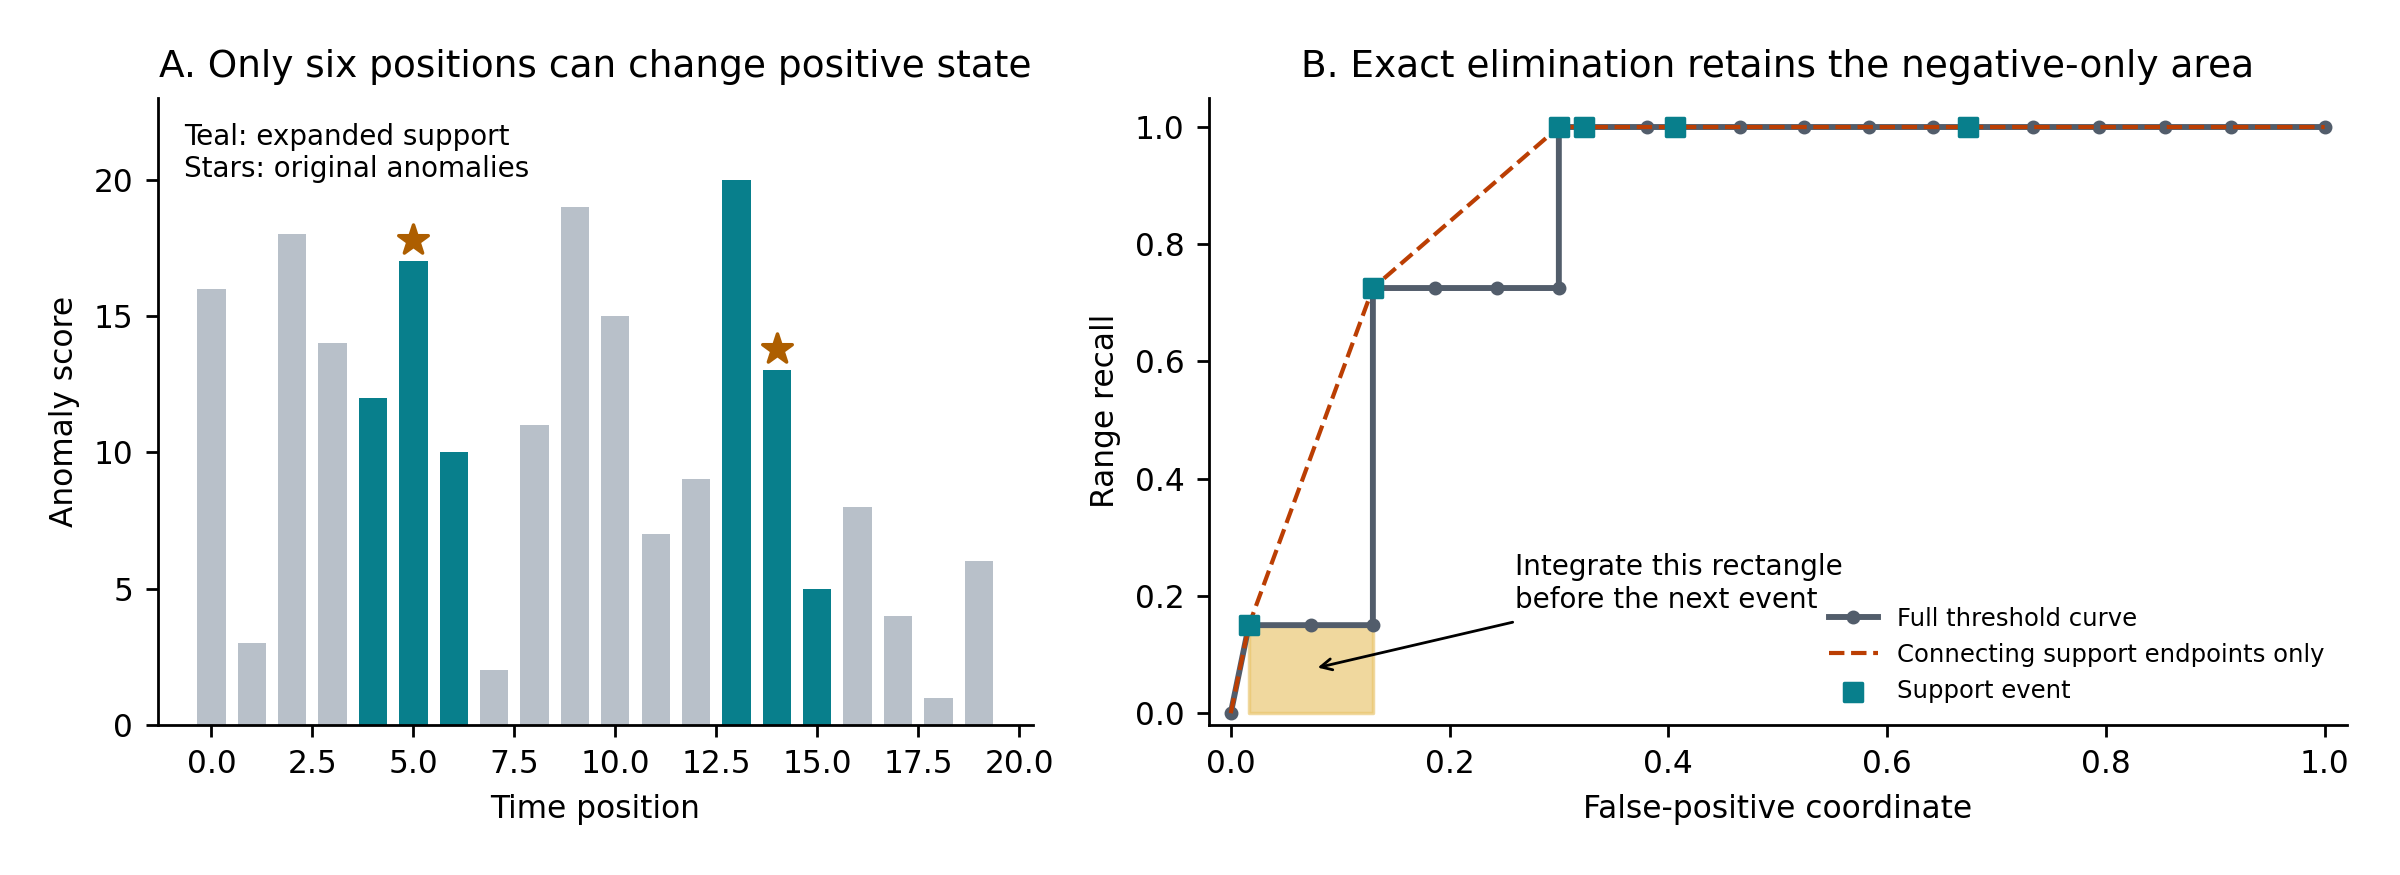
\includegraphics[width=0.94\linewidth]{figures/event-elimination.png}
\caption{A width-two example. Negative-only thresholds move horizontally
along the ROC curve. Integrating these rectangles and the subsequent tied
support transitions preserves the full-threshold area (0.841642); joining
support endpoints alone gives 0.897580.}
\label{fig:events}
\end{figure}

\begin{lemma}[Two interval distances]
For a non-original position, the official buffer weight is determined by its
two nearest distinct anomaly intervals.
\end{lemma}
\begin{proof}
Each active ramp contributes at least $\sqrt{1/2}$. If at least two intervals
contribute, their sum exceeds one and clipping returns one. Otherwise the
unique contribution is determined by the nearest interval. Hence the weight
is zero when $d_1>\lfloor w/2\rfloor$, one when
$d_2\le\lfloor w/2\rfloor$, and $\sqrt{1-d_1/w}$ otherwise. Original positive
positions remain one. The nearest two distances are computed from the two
neighboring intervals on either side in sorted interval order.
\end{proof}

\begin{theorem}[Support-sensitive exact evaluation]
The two pinned scalar VUS integrals can be computed in
$O(n\log(Q+1)+(L+1)Q)$ time and $O(n+Q)$ memory in a unit-cost real-arithmetic
model with score comparisons and square roots.
The returned values equal the reference integrals in exact arithmetic.
\end{theorem}
\begin{proof}
Extract intervals and $S_L$ in $O(n+Q)$ time. Sort the $Q$ support scores and
group their $G$ distinct values. Binary-search each of the $n$ scores among
these values and accumulate counts to obtain every $c_j^>,c_j^\ge$, without
sorting off-support scores. This costs $O(Q\log Q+n\log(G+1))$, bounded by
$O(n\log(Q+1))$ because $1\le G\le Q\le n$. Precomputing the two nearest
interval distances costs $O(Q\log(K+1))$, absorbed by the same bound since
the number of original intervals $K\le Q$.

For each width, construct weights in $O(Q)$ using Lemma 2. Assign disjoint
expanded interval memberships in $O(Q+K)$ and find each interval's earliest
support-score group. Grouped weighted sums and cumulative sums yield $\TP$,
$B$, and $H$ for all $G$ events in $O(Q+G+K)=O(Q)$ time. Lemma 1 and the
event formulas reproduce every omitted threshold contribution, including the
terminal tail. Average over $L+1$ widths. Arrays for the input, a position map,
support positions, grouped states, and interval metadata require $O(n+Q)$
memory. Floating-point implementations approximate this exact-arithmetic
identity; their numerical error is measured separately.
\end{proof}
The compiled scalar kernel streams the width average. The NumPy diagnostic
implementation retains per-width areas and uses an additional $O(L)$ space.
For dense support, $Q=\Theta(n)$, no asymptotic improvement over a dense sweep
is promised. The analysis establishes an upper bound.

\subsection{Linear preparation for fixed-width scores}
\label{sec:radix}
The comparison-based preparation can be replaced when scores have the
artifact's finite IEEE-754 binary64 representation. Counting radix sort is
standard~\cite{demaine2011radix}; order-preserving floating-point bit
transforms also predate this work~\cite{herf2001radix}. We combine these
existing techniques with the exact support-event representation and a linear
interval sweep. This is a VUS-specific composition, not a new sorting method.

After the public Float64 conversion, normalize both signed zeros to the
positive-zero bit pattern. Let $u$ be the resulting unsigned 64-bit word and
$h=2^{63}$. Form an ascending key by complementing every bit when the sign
bit is set, and by XOR with $h$ otherwise; complement this key for descending
score order. Eight stable counting passes, from the least to the most
significant byte, sort position indices using 256 buckets per pass. No
comparison-sort library dispatch is assumed.

Scan the resulting permutation by complete global tie groups. A group
containing a support position becomes one retained event; its starting and
ending ranks give $c_j^>$ and $c_j^\ge$. All support positions in that group
receive its event index. A group containing no support position advances the
global rank without creating an event. Consequently off-support points tied
with a support score enter together with that score, rather than being
mistakenly charged to the preceding negative-only rectangle.

For geometry, scan the temporally ordered support positions with a pointer
to the first original interval whose start exceeds the current position.
Inspect the two immediately preceding and two immediately following
intervals, when present, and retain the two smallest distances. Advancing
the pointer over all support positions takes $O(Q+K)$ time, where $K$ is the
number of original anomaly intervals.

\begin{proposition}[Fixed-width score preparation]
\label{prop:radix}
For finite binary64 score keys, assume unit-cost word operations, addresses
and counts that fit a machine word, and unit-cost metric arithmetic including
square roots. Preparation takes $O(n+Q+K)$ time. Exhaustive evaluation of
either scalar PR or the ROC--PR pair takes $O(n+(L+1)Q)$ time and preserves
the target integrals in exact metric arithmetic. The paired implementation
uses $O(n+Q)$ auxiliary words; the current PR-only implementation uses
$O(n+Q+L)$ because it retains one scalar per width.
\end{proposition}
\begin{proof}
For nonnegative finite binary64 values the unsigned bit patterns increase
with numerical value; for negative values their magnitude order is reversed.
The sign-dependent transform therefore preserves numerical order, and the
final complement reverses it. Canonicalizing zero makes key equality
equivalent to numerical equality on the validated finite domain. Stability
of each counting pass preserves the previously sorted lower bytes, so eight
passes give the complete descending order in $O(8(n+256))$ time. The tie scan
then obtains the exact global counts and support groups in $O(n+Q)$ time.

Original intervals are disjoint and ordered. Among intervals starting at or
before a position, distance cannot decrease when moving farther left; among
those starting after it, distance cannot decrease when moving farther right.
Thus two neighbors from each side contain two nearest distinct intervals,
including the possible interval containing the position. The monotone
pointer advances at most $K$ times. The two-distance lemma gives the same
summed-and-clipped weights at every width.

The remaining width kernel is unchanged: it processes $Q$ support positions,
$G$ score events and at most $K$ intervals per width. Since $G,K\le Q$, its
total cost is $O((L+1)Q)$. The exact event formulas preserve the omitted
negative thresholds and the terminal ROC transition. Input-sized keys,
permutation, scratch and position-map arrays require $O(n)$ words; support
and interval state requires $O(Q)$ more. The paired kernel streams the width
sum, whereas the PR-only completion interface stores $L+1$ scalar values.
\end{proof}

This bound uses a fixed 64-bit key universe; it is not a comparison-model
claim for arbitrary real scores or a bit-complexity bound for growing score
precision. Float64 conversion defines the threshold ties, including those
created when distinct large integers convert to the same score. The key and
count construction is discrete; subsequent floating-point accumulation has
the same numerical, rather than symbolic, exactness limitations as the
preceding evaluators.


\subsection{Matched dense execution controls}
The PR-only sparse implementation evaluates every width in one compiled
call, reusing scratch arrays and returning the mean scalar area. Its dense
controls also include validation, Float64 conversion, interval extraction,
global radix ranking, and every width in their public calls. One constructs
the original sum-and-clip ramps directly. The other computes the same two
nearest interval distances for all $n$ positions and uses the same weight
formula, retaining a full-rank PR-only sweep. Both complete global numerical
ties, reuse width scratch, and avoid ROC work, support-event compression,
and adaptive stopping. The nearest control takes $O((L+1)n)$ time and
$O(n+K)$ auxiliary memory. Thus the comparison does not attribute generic
radix, geometry, or single-metric savings to sparse support elimination.

\section{Prior art and implementation comparisons}
Boniol et al. introduce optimized VUS implementations with static/dynamic
label splitting, maximum-buffer support restriction, and memory tradeoffs
\cite{boniol2025}; these are substantive prior optimizations.
Klein's Apache-2.0 fast-VUS implementation, first committed on 12 October
2026, computes support-score cumulative sums, globally sorts all scores, and
evaluates the selected thresholds at every width \cite{klein2026}.
At audited revision \texttt{1bae859f}, passing \texttt{thre=n} gives full-threshold
PR with the target's dynamic mass, sum-and-clip ramps, expanded-interval
existence reward, and right-endpoint integration. Its API returns PR only;
the original measured API computes ROC and PR together, while the follow-up
also includes a PR-only kernel. Default 250-threshold and
full-threshold calls are distinguished in every comparison.
We do not claim support restriction, sorting support scores, or cumulative
sums as new. The remaining exact reduction removes inactive threshold events,
including their ROC contribution. The comparison-based preparation obtains
prediction counts without globally sorting all scores; the fixed-width
variant instead obtains them in a linear global radix pass.
Optional width enclosures are developed separately in
Appendix~\ref{sec:width}.

Sylligardos reports preliminary VUS speedups up to two
orders on CPU and three on GPU over approximately 1,900 TSB-UAD series
\cite{sylligardos2025}. Our expanded 21 October audit located attributed
FF-VUS NumPy/Torch code in the aVUSi repository, revision
\texttt{facf4362} \cite{ffvus2026}; the code is not linked by an immutable
receipt to that workshop figure. Its native linear, maximum-combined ramps
differ from the target's square-root, sum-and-clip ramps. The public wrapper
also rounds scores to two decimals, and Torch can interpolate intermediate
existence values when its memory estimate exceeds a threshold. For labels
$(0,1,0)$ and scores $(.101,.102,.001)$ at width zero, wrapper-equivalent
rounding changes PR from $1$ to $0.5$. A separate seven-point witness shows
a ramp mismatch even after matching physical radius. These are semantic
audits of unchanged code, not GPU timing comparisons. We do not claim the
first fast VUS implementation or superiority over all CPU/GPU variants.

The Benchopt time-series foundation-model benchmark supplies another
exact-compatible implementation, revision \texttt{2b55ccb1}, whose VUS
functions were introduced in May 2026 \cite{benchopt2026}. It globally sorts
scores, constructs full-array ramps, accumulates sorted masses, and obtains
existence through segment maxima and binary searches. Its unchanged
numerical function bodies return both ROC and PR; \texttt{thre=n} selects
the full-threshold target. We include it as an external dense-cumsum
comparator in the follow-up study, distinct from our independently written
dense controls.

The released Go \texttt{adscore} package implements an incremental dense rank
sweep \cite{boxer}. Native execution of its unmodified v0.0.23 package confirms
different semantics: static positive mass, original-interval existence,
maximum-combined overlapping ramps, and trapezoidal PR. On
$y=(0,1,0,0,1,0)$, $s=(1,2,3,4,5,6)$, and $L=4$, its ROC/PR values are
$(0.635984,0.638587)$, versus $(0.689265,0.683409)$ for the pinned target.
It is prior art for rank sweeps, but not an interchangeable exact-target
runtime baseline.

Current dtaianomaly commit \texttt{557b4357} provides a compiled, parallel
support-scan implementation with the target semantics \cite{dtaianomaly}.
We execute its original method bodies and compiled kernel unchanged through a
dependency-isolating adapter, obtain both integrals from one curve calculation,
and use one thread. Its support restriction differs from eliminating entire
negative-only threshold runs and aggregating all support events in one pass.
Both default 250-threshold and full-threshold variants are evaluated.

P-box lower and upper expectations for nonmonotone functions are established
by Utkin and Destercke \cite{utkin2009}; Troffaes and Destercke develop p-box
inference on totally preordered spaces \cite{troffaes2011}.
Our application uses the ordered support-event index as the state space and
endpoint recall as CDF bounds. The VUS-specific work is the merge partition,
coordinate-order proof, and adaptive integration over integer widths.
The source audit located no disclosed VUS algorithm with these width
enclosures, but this bounded search does not establish priority.

\section{Experimental protocol}
\subsection{Matched PR-only protocol and policy holdout}
The follow-up separates exact event compression from implementation choices
shared with dense methods. Its v3 protocol evaluates all three model scores
per series, returning every model within $10^{-10}$ of the maximum exact PR.
The 308 series outside the fixed 42-series development selection give 924
tasks at $L\in\{30,100,300\}$. They are held out for this procedure, not newly
collected data: the same corpus appeared in earlier experiments. The main
width is 30; widths 100 and 300 characterize wider-buffer regimes, with 300
an explicit stress condition.

Fourteen required methods include the comparison-based and radix sparse
evaluators, PR-only direct and nearest dense radix controls, released Klein
and Benchopt code, and the optional selection engines. Every timed call
includes preparation, all model evaluations or refinement, and winner-set
construction. Source loading, warmed imports/JIT compilation, and receipt
serialization are outside the measured interval. Three repetitions use
independent seeded random method order within each task and one compute
thread. Width-major task order, source hashes, required comparisons, and
family-bootstrap summaries are fixed by the protocol.

The matched dense controls and the v3 protocol were fixed after the v2
development results and before inspection of the policy-holdout outcomes.
The exact radix and radix racing hypotheses have separate decisions; each
requires correctness and favorable lower 95\% family-bootstrap bounds for
both geometric-mean ratios and ratios of summed task-median runtimes
against its required controls. These sums are not measured batch wall
times; the intervals describe family variation, not uncertainty from three
timing repetitions. The artifact preserves the amendments, complete v2 records and
original auditor. V2 and v3 timings are not pooled. These comparisons do not
claim global CPU/GPU state of the art.

\subsection{Earlier correctness and corpus studies}
The protocol, exact source hashes, score archive selection, and a pre-outcome
addendum are included with the artifact. The dtaianomaly comparator was selected
before execution; a separate, retrospectively written addendum records that
decision and its timing. One thousand independently seeded
random cases vary length, label density, ties, constant scores, and buffer
width; six structured cases cover edges and overlapping/adjacent expansions.
Separately authored validation scripts add 1,960 exhaustive tiny cases and 120 new random
cases, including extreme finite scores and arbitrary boundary labels.

We use three released score archives from Zhu et al. \cite{zhu2026}: Chronos-Bolt
base, Time-MoE 200M, and TimesFM 1.0 200M, each at context length 64. Models were
chosen by a frozen family/context/lexicographic rule. All common valid series
from the 350-series TSB-AD-U evaluation split \cite{tsbad} are included; no model is trained
or queried. Scores are read unchanged. Their source README documents leading
zero padding for Chronos-Bolt and Time-MoE; we do not reproduce that paper's
corrected model leaderboard. Original dataset licenses vary, and raw data and
scores are not redistributed.

The original corpus experiment evaluates maximum widths 10 and 30. Each timing includes
validation, preprocessing, sorting or histogramming, and integration. Three
repetitions use a seeded randomized method order; JIT compilation/first-call
time and downloads are excluded and recorded separately. The machine is an
\MachineCPU{}, Python \PythonVersion{}, with all compute libraries restricted
to one thread. We compare NumPy sparse, Numba sparse, NumPy dense, Numba dense
with precomputed nearest distances, and a separately implemented Numba dense
method constructing every original sum-and-clip ramp directly. Its principal
speed ratio uses the fastest median among all three dense implementations for
each input, favoring the dense baselines.

The final timed output for each full trace is cross-checked between all five
implementations. Official
full-threshold and sampled-threshold equivalence are checked on fixed
256-position crops around each first anomaly, when both classes occur.
Published external runtimes are measured on the prespecified first 12 common
series (all NAB, lengths 1,000--10,319), with all three score vectors and both
widths. Official 250-threshold timing has one repetition; dtaianomaly has three.
The five in-repository methods use randomized order. External methods use the
fixed order official-250, dtaianomaly-250, then dtaianomaly-exact. This external
timing subset is not representative of all dataset families.

Two supplementary protocols were fixed after review of the main setup and
before their respective executions. A mechanism ablation replaces only the
score-count preprocessing with a global full-score sort, then calls the
identical compiled sparse integration kernel. It crosses two lengths
($10^4,10^5$), four positive densities ($0.001,0.01,0.1,0.5$), four interval
counts ($1,10,100,1000$), and four maximum widths ($0,10,30,100$). Sixteen
geometrically infeasible cells are excluded before execution, leaving 112
cases. Five implementations run in randomized order for three repetitions.
The second supplement tests the actual published implementation across source
families; its selection and censoring rules are reported with the results.

For sampling effects, all three unordered model pairs per series/width are
examined. A reversal requires opposite signs and absolute metric differences
above $10^{-10}$ in both calculations; ties are reported separately. Series,
not score vectors or width/model repetitions, are the units for uncertainty
summaries. These are changes in ordering induced by metric computation, not
claims that one model is superior.

The padding sensitivity protocol was fixed after observing the original
results and padding inventory, before evaluating its transformations.
For Chronos-Bolt and Time-MoE, \emph{first-score fill} replaces the first
64 scores with the score at index 64, retaining full labels and all TimesFM
scores. \emph{Common suffix} evaluates positions 64 onward for every model.
Both interventions use the same 350 series, model pairs, and widths.
The suffix changes prevalence, threshold ranks, and boundary geometry;
21 series contain positive labels in the removed prefix. Neither intervention
reconstructs every preprocessing choice in the source model paper.

\section{Results}
% BEGIN V3 RESULTS: the measurement owner supplies the audited fragment.
\IfFileExists{pr_engine_results.tex}{\subsection{Frozen v3 policy holdout: exact radix evaluation}
\label{sec:pr-engine-results}
Each platform completed all 924 tasks on the same 308 series in 17 families,
with $L=30$ primary, $L=100$ secondary, and $L=300$ a stress regime.
Each task evaluates the three frozen model score vectors and returns the best-PR model set, retaining numerical ties.
Times include whole-task preparation and use the median of three repetitions.
The maximum absolute PR discrepancy from the comparison-sort sparse PR reference was
$1.554\times 10^{-15}$ on Mac and $1.332\times 10^{-15}$ on Linux.
These are numerical agreement checks for the pinned target.

The frozen exact-radix decision at $L=30$ is Mac: \textbf{PASS}; Linux: \textbf{PASS}.
It requires both the geometric-mean and aggregate-ratio lower confidence bounds
to exceed one against every one of the five frozen controls, together with correctness.
Klein and Benchopt comparisons are descriptive and are outside this decision.
Table~\ref{tab:radix-primary} retains every primary control and both external implementations.

All ratios are comparator time divided by exact sparse-radix PR time; values above one favor radix PR.
Brackets contain audited 95\% family-cluster bootstrap intervals (2000 resamples).
The aggregate ratio divides sums of per-case median times; it is not an observed batch wall time.
Intervals describe variation across families, not uncertainty in three timing repetitions.
F/S/T counts cases where radix PR is faster/slower/tied. Decisions use unrounded bounds.

\begin{table}[tbp]
\centering\small
\setlength{\tabcolsep}{3pt}
\caption{Primary $L=30$: all 308 cases per platform. $\dagger$ marks the five frozen decision controls. R+P methods compute both ROC and PR; the others compute PR only. Dense direct and dense nearest use comparison sorting unless labelled radix.}
\label{tab:radix-primary}
\resizebox{\linewidth}{!}{%
\begin{tabular}{llrrrr}
\toprule
Platform & Comparator & Median & Geomean [CI] & Aggregate [CI] & F/S/T \\
\midrule
Mac & Sparse comparison$^{\dagger}$ & 1.774 & 1.620 [1.421, 1.920] & 1.960 [1.511, 2.323] & 271/37/0 \\
Mac & Dense direct$^{\dagger}$ & 3.331 & 3.160 [2.772, 3.506] & 4.255 [3.349, 5.112] & 306/2/0 \\
Mac & Dense nearest (R+P)$^{\dagger}$ & 5.050 & 4.840 [4.356, 5.368] & 6.140 [4.974, 7.181] & 308/0/0 \\
Mac & Dense direct radix$^{\dagger}$ & 2.677 & 2.617 [2.318, 2.870] & 3.595 [2.752, 4.514] & 303/5/0 \\
Mac & Dense nearest radix$^{\dagger}$ & 2.599 & 2.519 [2.297, 2.726] & 3.298 [2.624, 3.980] & 307/1/0 \\
Mac & Klein fast-VUS & 20.925 & 22.360 [19.764, 24.238] & 19.450 [17.910, 20.623] & 308/0/0 \\
Mac & Benchopt (R+P) & 35.420 & 37.572 [34.754, 41.101] & 37.990 [34.728, 42.965] & 308/0/0 \\
\midrule
Linux & Sparse comparison$^{\dagger}$ & 1.987 & 1.916 [1.839, 2.013] & 1.955 [1.745, 2.095] & 304/4/0 \\
Linux & Dense direct$^{\dagger}$ & 4.894 & 4.161 [3.170, 5.008] & 5.385 [4.241, 6.191] & 308/0/0 \\
Linux & Dense nearest (R+P)$^{\dagger}$ & 6.917 & 5.890 [4.639, 6.923] & 7.214 [5.688, 8.187] & 308/0/0 \\
Linux & Dense direct radix$^{\dagger}$ & 4.419 & 3.756 [2.904, 4.486] & 4.708 [3.794, 5.276] & 308/0/0 \\
Linux & Dense nearest radix$^{\dagger}$ & 4.791 & 4.047 [3.142, 4.821] & 5.010 [3.933, 5.643] & 306/2/0 \\
Linux & Klein fast-VUS & 14.538 & 13.814 [11.639, 15.930] & 11.232 [10.034, 12.514] & 308/0/0 \\
Linux & Benchopt (R+P) & 21.493 & 20.973 [18.481, 23.617] & 22.991 [19.193, 30.937] & 308/0/0 \\
\bottomrule
\end{tabular}}
\end{table}

\paragraph{Secondary and stress regimes.}
Table~\ref{tab:radix-secondary} gives both matched PR-only radix dense controls at $L=100$ and $L=300$.
These controls share fixed-width score ordering with sparse radix and retain full dense width sweeps.
Their ratios assess the support-event reduction after matching the ranking implementation.
The full bound reports retain every other comparator, family effect, and slower case at each width.

\begin{table}[tbp]
\centering\small
\setlength{\tabcolsep}{3pt}
\caption{Secondary and stress widths: all 308 cases per row, matched PR-only controls. Ratio direction and intervals follow Table~\ref{tab:radix-primary}.}
\label{tab:radix-secondary}
\resizebox{\linewidth}{!}{%
\begin{tabular}{lllrrrr}
\toprule
Platform & $L$ & Comparator & Median & Geomean [CI] & Aggregate [CI] & F/S/T \\
\midrule
Mac & 100 & Dense direct radix & 5.110 & 4.834 [3.728, 5.802] & 6.874 [4.488, 8.943] & 307/1/0 \\
Mac & 100 & Dense nearest radix & 4.637 & 4.551 [3.602, 5.370] & 6.096 [4.117, 7.577] & 305/3/0 \\
Mac & 300 & Dense direct radix & 6.916 & 6.534 [4.259, 8.903] & 8.850 [5.163, 12.681] & 308/0/0 \\
Mac & 300 & Dense nearest radix & 6.294 & 6.000 [3.902, 8.163] & 7.892 [4.670, 11.080] & 300/8/0 \\
Linux & 100 & Dense direct radix & 7.465 & 6.666 [4.438, 8.952] & 8.220 [5.435, 10.714] & 308/0/0 \\
Linux & 100 & Dense nearest radix & 7.919 & 6.975 [4.574, 9.447] & 8.543 [5.360, 11.345] & 302/6/0 \\
Linux & 300 & Dense direct radix & 7.612 & 7.360 [4.333, 10.986] & 8.808 [5.506, 13.079] & 308/0/0 \\
Linux & 300 & Dense nearest radix & 8.103 & 7.426 [4.155, 11.417] & 8.943 [5.047, 13.692] & 295/13/0 \\
\bottomrule
\end{tabular}}
\end{table}

\paragraph{Post-protocol descriptive PR-only oracle.}
For each case, the oracle selects the fastest of comparison-based sparse PR, direct dense PR,
Klein PR, direct dense radix PR, and nearest-interval dense radix PR.
Paired ROC+PR methods and adaptive racers are excluded from this PR-only exhaustive set.
Table~\ref{tab:radix-oracle} and Figure~\ref{fig:radix-oracle} retain every case and loss.
No confidence interval is assigned to this retrospective minimum, and it changes no frozen decision.

\begin{table}[tbp]
\centering\small
\setlength{\tabcolsep}{3pt}
\caption{Descriptive PR-only oracle / exact sparse-radix ratios; no confidence intervals. Minimum retains the slowest relative radix case.}
\label{tab:radix-oracle}
\resizebox{\linewidth}{!}{%
\begin{tabular}{llrrrrr}
\toprule
Platform & $L$ & Median & Geomean & Aggregate & F/S/T & Minimum \\
\midrule
Mac & 30 & 1.709 & 1.582 & 1.924 & 268/40/0 & 0.531 \\
Mac & 100 & 1.557 & 1.500 & 1.734 & 286/22/0 & 0.618 \\
Mac & 300 & 1.278 & 1.293 & 1.375 & 285/23/0 & 0.610 \\
Linux & 30 & 1.986 & 1.879 & 1.928 & 302/6/0 & 0.807 \\
Linux & 100 & 1.715 & 1.655 & 1.612 & 301/7/0 & 0.815 \\
Linux & 300 & 1.275 & 1.309 & 1.235 & 294/14/0 & 0.770 \\
\bottomrule
\end{tabular}}
\end{table}

\begin{figure}[tbp]
\centering
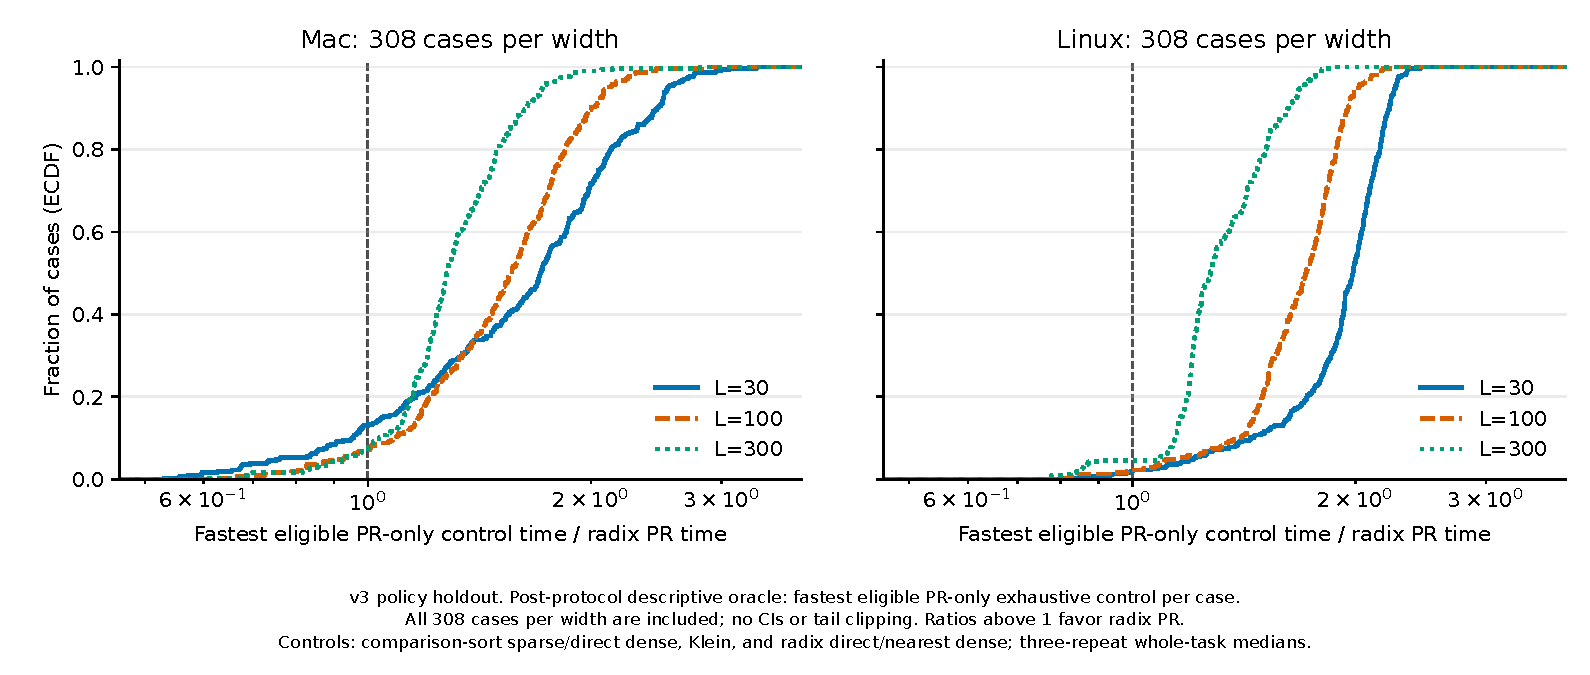
\includegraphics[width=\linewidth]{figures/pr-only-oracle-ecdf.pdf}
\caption{Post-protocol oracle ECDFs for the v3 policy holdout: all 308 cases at each width on each platform, without tail clipping. The horizontal coordinate is the fastest eligible exhaustive PR-only control's whole-task case median divided by exact sparse-radix PR time. Values above one favor radix PR. The five eligible controls are specified in the text; no oracle confidence intervals are computed.}
\label{fig:radix-oracle}
\end{figure}

\paragraph{Separate racing decisions and scope.}
The frozen comparison-order racing decision at $L=30$ is Mac \textbf{FAIL}, Linux \textbf{FAIL}; the separate radix-order racing decision is Mac \textbf{FAIL}, Linux \textbf{FAIL}.
The first requires both interval lower bounds above one against comparison-based sparse PR, direct dense PR, and exact radix PR;
the second additionally requires this against both matched dense radix PR controls.
These decisions include preparation, adaptive queries, and exact completion in each measured task.
Racing outcomes are separate from the exact-radix decision, and failed criteria remain reported.
The v2 development runs remain historical development evidence and are not pooled with this holdout.
Platforms are summarized separately: no cross-run timing pooling is performed.
The Mac was not isolated: its starting snapshot shows an unrelated Python worker near 100 percent CPU, alongside normal desktop activity. Snapshots are not a continuous load trace. Agent test, build, and report execution stopped during timing; lightweight status reads, completed remote-artifact transfers, and document edits continued. No unrelated process was stopped by the experiment.
The Linux confirmation used a separate serial GitHub Actions job; hosted hardware and host background load were outside our control.
This policy holdout uses previously studied corpus families; it is not an external-domain dataset.
The results address the stated workload and tested implementations, without establishing universal superiority.

\par\noindent{\footnotesize Reproducibility receipt (SHA-256 prefixes): Mac report \texttt{c72f2df666c4}, audit \texttt{a9d44deb51fa}; Linux report \texttt{46c6fba361e4}, audit \texttt{577dab610dd4}. The accompanying JSON receipt records full report, measured-source, and generator hashes.}
}{}
% END V3 RESULTS

The following exact benchmark predates the fixed-width radix implementation.
It measures individual score-vector calls at widths 10 and 30, separately
from the v3 three-model PR-selection workload. Its results are retained as
corroborating evidence for the earlier comparison-based event reduction;
they are not measurements of the new radix kernel or pooled with v3 ratios.
% Measured source: artifacts/advancement/analysis/analysis.json
% SHA-256: 3727de01958ef96deb0c15ad22823506eb9097e975f046334d84976a10e37762
\subsection{Exact evaluation against released fast-VUS on two machines}
A new complete run compares the unchanged fast-VUS module at full thresholds
against Sparse VUS and the three dense implementations. Each machine evaluates
all 2,100 original model/width cases on 350 series from 23 families. Each call
includes validation, preprocessing, and integration; three repetitions use
randomized method order, one compute thread, and excluded JIT warmup.
The M1 Pro run uses Python 3.12.4, NumPy 1.26.4, and Numba 0.59.1.
The Linux hosted runner identifies an AMD EPYC 9V74 and uses Python 3.12.15,
NumPy 2.5.4, and Numba 0.68.0. Ordinary OS and hosted-hardware background load
is uncontrolled. The Linux run is a separate execution, not an external
laboratory reproduction.

Table~\ref{tab:fast-vus} reports within-machine ratios. Fast-VUS returns only
PR; Sparse VUS computes both ROC and PR. The per-case fastest-tested comparator
is the minimum median runtime among fast-VUS and all three dense evaluators,
excluding Sparse VUS itself. This is an oracle comparison, not a deployable
selector. The maximum PR difference from fast-VUS is $2.78\cdot10^{-15}$;
the largest discrepancy across all exact methods is $3.70\cdot10^{-13}$.

\begin{table}[t]
\centering
\begin{tabular}{llrrrr}
\toprule
Machine & Comparator & Median & \shortstack{Geometric mean\\(95\% interval)} & Faster & \shortstack{Slower\\or equal}\\
\midrule
M1 Pro & fast-VUS & 8.38 & 8.69 [8.32, 9.05] & 2100 & 0 \\
M1 Pro & Fastest tested & 2.04 & 1.98 [1.89, 2.07] & 1891 & 209 \\
EPYC 9V74 & fast-VUS & 4.55 & 4.50 [4.34, 4.68] & 2100 & 0 \\
EPYC 9V74 & Fastest tested & 1.35 & 1.40 [1.34, 1.46] & 1526 & 574 \\
\bottomrule
\end{tabular}
\caption{Comparator runtime divided by Sparse VUS runtime; values above one
favor Sparse VUS. Every row covers 2,100 cases. Intervals resample whole series
and describe geometric means on the fixed corpus. Both methods use all
thresholds; fast-VUS computes PR only.}
\label{tab:fast-vus}
\end{table}

Fast-VUS ratios range from 1.75 to 46.45 on M1 Pro and 1.52 to 17.97 on Linux.
Against the fastest-tested comparator, ranges are 0.40--7.75 and 0.36--8.40.
Whole-family bootstrap intervals for the latter geometric means are
[1.53,2.42] and [1.11,1.68], respectively. The corpus and machines support a
bounded measured advantage, with substantial dense-baseline slowdown cases;
they do not settle the unavailable Sylligardos comparison.
The sums of isolated per-case medians are 14.78 versus 104.52 seconds for
Sparse VUS and fast-VUS on M1 Pro, and 14.39 versus 55.14 seconds on Linux.
These sums are not measured batch or detector-pipeline wall times.

\subsection{Error bounds and the cost of width refinement}
The width-refinement experiment retains the metadata-selected 42 series
covering all 23 families and all three released score vectors. Maximum widths
30, 100, and 300 give 378 model/width cases; the width-300 setting is an
explicit stress condition. Both $\varepsilon=0.01$ and $0.001$ bound the
half-widths of both returned metric intervals. The M1 Pro timing protocol
again includes whole-call preprocessing and uses three randomized-order
repetitions. Table~\ref{tab:width-refinement} compares against full-width
Sparse VUS on these same inputs.

\begin{table}[t]
\centering
\begin{tabular}{rrrrrr}
\toprule
$\varepsilon$ & $L$ & \shortstack{Median\\ratio} & Faster / 126 & \shortstack{Distinct\\widths (\%)} & \shortstack{Curve calls\\(\%)}\\
\midrule
0.01 & 30 & 0.835 & 27 & 16.1 & 16.1 \\
0.01 & 100 & 0.905 & 46 & 7.9 & 7.9 \\
0.01 & 300 & 1.313 & 100 & 4.7 & 7.3 \\
0.001 & 30 & 0.615 & 4 & 54.8 & 80.6 \\
0.001 & 100 & 0.426 & 11 & 39.6 & 74.3 \\
0.001 & 300 & 0.391 & 25 & 25.4 & 53.8 \\
\bottomrule
\end{tabular}
\caption{Full-width exact runtime divided by adaptive runtime. Width and
curve-call columns are medians relative to $L+1$; cache eviction can make
curve calls exceed the number of distinct widths. Values below one indicate
that adaptive evaluation is slower.}
\label{tab:width-refinement}
\end{table}

All 378 cases at both tolerances contain the full-width ROC and PR values
within the separately declared $10^{-10}$ numerical audit allowance.
Maximum midpoint errors are $0.003260$ and $0.000713$ for tolerances 0.01
and 0.001. However, fewer width evaluations do not generally imply faster
execution. Across all three maximum widths, median runtime ratios are
0.966 and 0.467, with adaptive evaluation faster in 173 and 40 of 378 cases,
respectively. At tolerance 0.01 and $L=300$, the geometric mean ratio is
1.370 (series-bootstrap interval [1.207,1.557]); at the tighter tolerance,
all three width groups have geometric mean ratios below one.
The present implementation therefore provides useful enclosures, but the
standalone fixed-tolerance strategy is often slower than exact evaluation.

As a numerical decision replay, nonoverlapping PR intervals identify unique
winners in 21, 17, and 15 of the 42 series at tolerance 0.01 for widths
30, 100, and 300; the corresponding counts at tolerance 0.001 are 33, 32,
and 34. All asserted winners agree with exact PR using the declared
$2\cdot10^{-10}$ separation margin. These replay counts do not include
additional decision-workload timing or establish a model-selection speedup.

Separately authored validation directly constructs full-threshold curves
for every both-class binary label vector of lengths two through seven,
using four seeded score patterns per vector. It checks 13,776 widths and
width enclosures and 960 discrete averages. The largest curve discrepancy
is $6.67\cdot10^{-16}$ and the largest enclosure violation is
$3.34\cdot10^{-16}$, within the declared $2\cdot10^{-12}$ allowance.
A further 760 linear-programming comparisons of p-box extrema have maximum
discrepancy $3.34\cdot10^{-16}$. Exhaustiveness concerns labels only, not all
rankings or tie patterns; these checks audit the implementation and complement
the real-arithmetic proofs.



\subsection{Optional width reduction: fewer queries can cost more}
The support-event curves also admit merge-aware width enclosures using
established probability-box bounds. Their real-arithmetic guarantees and
numerical implementation allowances are distinct. In the earlier 378-case
study, fixed-tolerance refinement had median exact/adaptive runtime ratios
of 0.966 at tolerance 0.01 and 0.467 at tolerance 0.001. The ensuing
incremental racer agreed with exact decisions on all 126 development tasks
on both CPUs, but increased the sum of per-task median latencies even at
width 300, where its median speed ratio exceeded one. Fewer distinct width
queries therefore do not establish a practical acceleration. The compiled
PR-only follow-up and matched dense controls are separately specified and
measured; they do not erase the earlier negative results. Full proofs,
controller details, measurements, and development chronology are retained
in Appendices~\ref{sec:width} and~\ref{sec:racing}.

\subsection{Consequences of a fixed threshold grid}
In the original corpus experiment, the reference's 250-threshold grid
reverses 84 of 2,100 PR pair orders relative to exact evaluation. Most gaps
are small: only five reversals have both gaps at least 0.01. Two fixed
padding interventions retain 75 and 74 of the original reversals, while
also introducing other changed orders. Appendix~\ref{app:corpus} retains
the full original results, effect-size analysis, and padding sensitivity.
These are consequences of metric approximation, not evidence that one
detector is better or that VUS is the preferred selection criterion.

\section{Limitations and reproducibility}
The target is a specific, pinned scalar implementation. Exactness does not
resolve scientific criticisms of the underlying metric, extend it to all
historical variants, or produce the full surface. The acceleration depends on
sparse expanded support and can disappear for dense support. Adaptive bounds
can require all widths and add overhead; tolerance is not a guaranteed speedup.
Real-arithmetic enclosures and float64 checks are distinct: no machine-level
interval certificate or unconditional numerical ordering guarantee is claimed.
Floating-point equivalence is numerical, not bitwise. The NumPy/Numba dense implementations
are independently written algorithmic baselines, not published competing
systems. Published-code comparisons retain API and threshold-resolution
differences. The actual released dtaianomaly comparison is bounded, and the
located FF-VUS implementation computes a different native metric and is
audited semantically rather than ranked as an exact-compatible runtime baseline.

The artifact includes source, tests, derivations, frozen protocols, download
and source-checksum receipts, per-input timing and metric records, negative
results, and figure/manuscript regeneration scripts. Dated receipts identify
each CPU execution and protocol version; all use released scores and no
models are retrained. AI systems were used extensively in software
development, mathematical derivation,
experiment analysis, manuscript drafting, and in-session review.
Separate checks use distinct test implementations within this session,
not external laboratory reproduction.

\section{Conclusion}
Score groups containing no maximum-support position can be eliminated while
preserving their ROC rectangles and the complete ties at retained events.
Combining this exact representation with standard fixed-width ranking and
linear interval geometry gives $O(n+(L+1)Q)$ exhaustive evaluation under the
stated arithmetic model. The earlier comparison-based evaluator shows
measured gains over released fast-VUS on both tested CPUs, while dense
methods retain favorable cases. Matched PR-only dense radix controls are
necessary to distinguish support-event gains from shared implementation
improvements. Width enclosures and adaptive decisions remain optional:
their lower query counts alone do not justify replacing exhaustive exact
evaluation. The contribution concerns efficient computation of a specified
metric, not the validity of that metric or universal runtime superiority.

\appendix
\section{A fixed uniform-rank grid can lose almost all PR area}
\label{app:grid}
The following proposition concerns the particular uniform-rank sampling rule
used by the pinned reference, with all input scores distinct. It does not
apply to every adaptive threshold-selection scheme.

\begin{proposition}
Fix an integer threshold budget $T\ge2$, a maximum width $L\ge0$, and
$\varepsilon>0$. There are finite-score binary-label sequences for which the
absolute difference between exact VUS-PR and the reference's $T$-threshold
VUS-PR is greater than $1-\varepsilon$.
\end{proposition}
\begin{proof}
Take one anomaly interval of length $m$, with at least $\lfloor L/2\rfloor$
positions of padding on both sides. Give its original positives score ranks
$2,\ldots,m+1$, put the highest-scored point outside the maximum-width
support, and give all buffer positions the next consecutive ranks. Give all
other positions distinct lower scores. Append further lower-scored negatives
at the right, preserving the existing geometry and scores.

For every $w\le L$, the $j$th original positive is admitted before any buffer
point. Its recall is $j/m$, precision is $j/(j+1)$, and existence reward is
one. Recall reaches one after the last original positive. All subsequent PR
increments are zero, so exact VUS-PR is
\begin{equation}
 E_m=\frac1m\sum_{j=1}^m\frac{j}{j+1}
 =1-\frac{H_{m+1}-1}{m},
\end{equation}
where $H_k$ is the $k$th harmonic number.

The sampled grid has one-based ranks
$1+\lfloor j(n-1)/(T-1)\rfloor$, for $j=0,\ldots,T-1$.
For sufficiently large $n$, its second rank
$k_n=1+\lfloor(n-1)/(T-1)\rfloor$ contains all maximum-width support.
The first sampled recall is zero. Let $A_w=\sum_i a_i^{(w)}$ denote the full
label mass. At the second threshold, $\TP=A_w$, $B=A_w-m$, and
$P=(m+A_w)/2$. Thus clipped recall and existence reward both equal one,
and precision is $A_w/k_n$. No later sampled threshold adds PR area.
The sampled VUS-PR therefore equals
$\overline A/k_n$, where $\overline A=(L+1)^{-1}\sum_{w=0}^L A_w\le m+L$.

First choose $m$ so that $(H_{m+1}-1)/m<\varepsilon/2$; then append enough
negatives that $k_n$ exceeds all support ranks and
$2(m+L)/\varepsilon$. The exact area exceeds $1-\varepsilon/2$ and the
sampled area is less than $\varepsilon/2$, proving the claim.
\end{proof}
The artifact includes deterministic checks at $T=250$, $m\in\{1,10\}$,
$L\in\{0,6\}$, and $n\in\{10^4,10^5\}$ against the two closed-form values.
\section{Earlier corpus sampling and padding studies}
\label{app:corpus}
\subsection{Corpus-wide sampling effects and supporting measurements}
The original fixed-corpus run provides the following threshold-sampling
analysis and complementary dense-baseline measurements. These timings are
retained as a separate run; they are not pooled with the current published-code
comparisons.
The completed experiment contains 350 series from 23 source
families, 1050 released score vectors, and 2100 score/width
evaluations. Sequence lengths range from 1,000 to
900,000. The independent final artifact gate passes all
coverage, finite-value, source-hash, internal, crop, and external-comparator checks.
The maximum absolute numerical discrepancy is $3.69\times10^{-13}$.

The median compiled-sparse speedup over the fastest dense baseline is
2.06$\times$, with geometric mean 2.02$\times$.
The 95\% series-cluster bootstrap interval for the geometric mean is
[1.93, 2.12]; resampling whole source families gives
[1.56, 2.48]. These are descriptive uncertainty summaries
for the fixed corpus. Sparse evaluation is faster in 1916 of
2100 cases, while 184 cases are slower or equal.
The full speedup range is 0.27--7.50$\times$.
Figure~\ref{fig:results} retains these slowdowns rather than filtering dense support.

\begin{figure}[t]
\centering
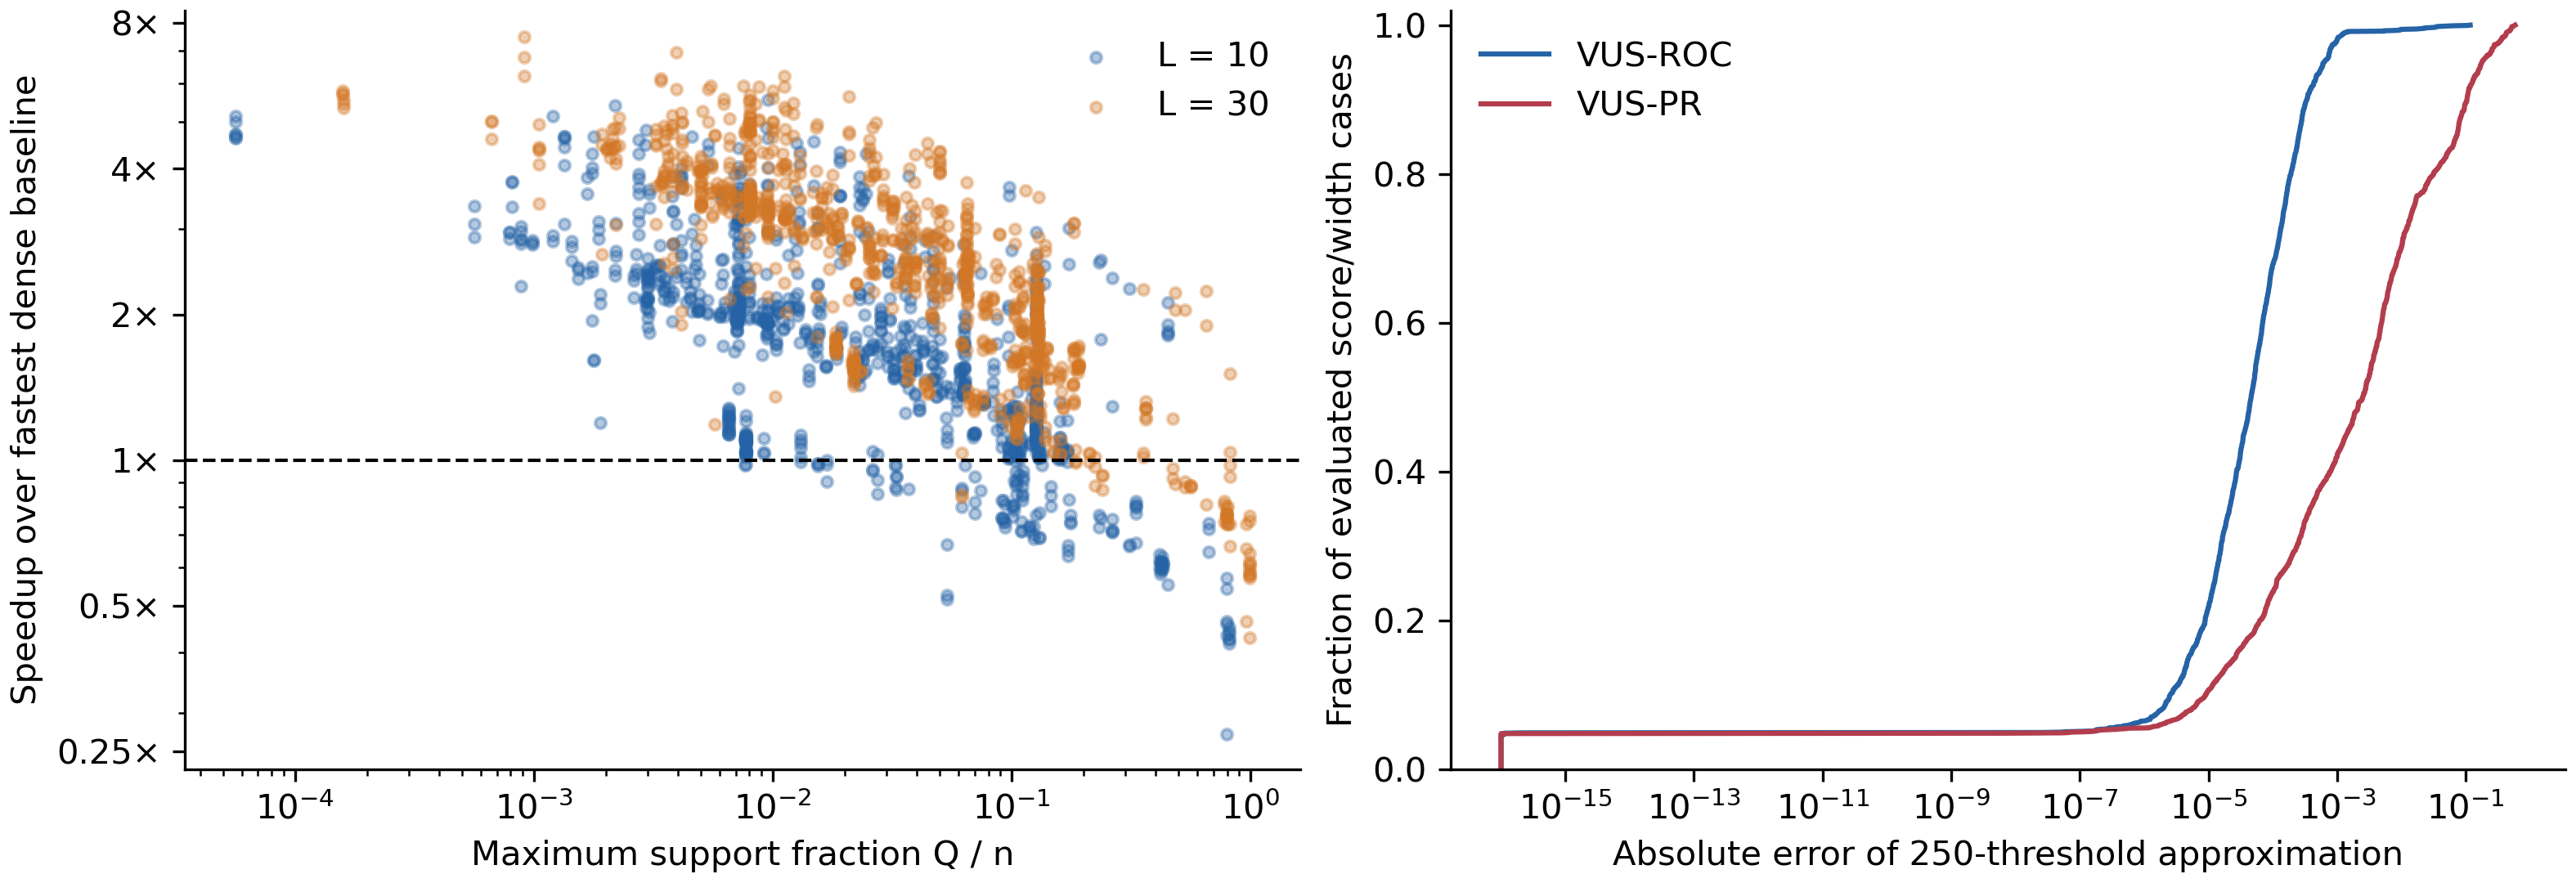
\includegraphics[width=\linewidth]{public-results.png}
\caption{Left: all 2100 paired runtime comparisons, using the fastest of three dense
implementations per input. Right: threshold-sampling error on the same fixed score vectors.
Zero errors are displayed at $10^{-16}$ for the logarithmic axis.}
\label{fig:results}
\end{figure}

\begin{table}[htbp]
\centering
\begin{tabular}{lrrrr}
\toprule
Metric & Median error & 95th percentile & Maximum error & Reversals / pairs \\
\midrule
VUS-ROC & $4.59\times10^{-5}$ & $6.21\times10^{-4}$ & $0.117$ & 5 / 2100 \\
VUS-PR & $2.50\times10^{-3}$ & $0.178$ & $0.583$ & 84 / 2100 \\
\bottomrule
\end{tabular}
\caption{Errors are absolute differences between the same metric at 250 sampled thresholds and all thresholds. Reversals require strict opposite order in both calculations.}
\label{tab:sampling}
\end{table}

For VUS-ROC, strict reversals occur on 2 unique series across 2 families, and the unique top model changes in 2 of 700 series/width cases. Exact and sampled comparisons contain 96 and 95 ties, respectively.

For VUS-PR, strict reversals occur on 55 unique series across 13 families, and the unique top model changes in 50 of 700 series/width cases. Exact and sampled comparisons contain 96 and 95 ties, respectively.

The largest observed PR discrepancy occurs on the 195,000-point UCR HumanActivity series with Time-MoE scores and $L=30$: exact VUS-PR is 0.666890, versus 0.084159 at 250 thresholds. The scores are unchanged between calculations.

On the bounded 12-series NAB external comparison, the median speed ratios relative to compiled sparse evaluation are 53.86$\times$ for full-threshold dtaianomaly, 8.92$\times$ for 250-threshold dtaianomaly, and 149.29$\times$ for official 250-threshold evaluation. The latter two compare exact computation with a coarser approximation. These results do not establish the same advantage on other families or against the unavailable accelerated VUS implementation.

In the frozen fixed-support scaling experiment ($Q=102$, $L=30$), the one-million-point case takes 0.0626 seconds for compiled sparse evaluation, an 8.92$\times$ speedup over the fastest dense implementation, with five randomized-order repetitions.

\subsection{Mechanism and the density/width tradeoff}
On the 112-case synthetic grid, replacing full-score sorting with
support-score counting gives a geometric-mean end-to-end speedup of
1.11$\times$ with the same integration kernel,
range 0.94--1.80$\times$.
The adapter deliberately holds support grouping and all other preparation
fixed, isolating the score-counting choice. Relative to the fastest dense
implementation, the complete sparse method has geometric-mean speedup
1.37$\times$, range
0.26--7.53$\times$.
There are 69 cases with at least a 1.1$\times$
speed ratio and 34 with ratio at most $1/1.1$.
The remaining cases lie between those thresholds. Thus the count-preprocessing
improvement is modest on this grid; sparse event integration supplies the
larger opportunity as support shrinks and the width range grows.

\begin{figure}[t]
\centering
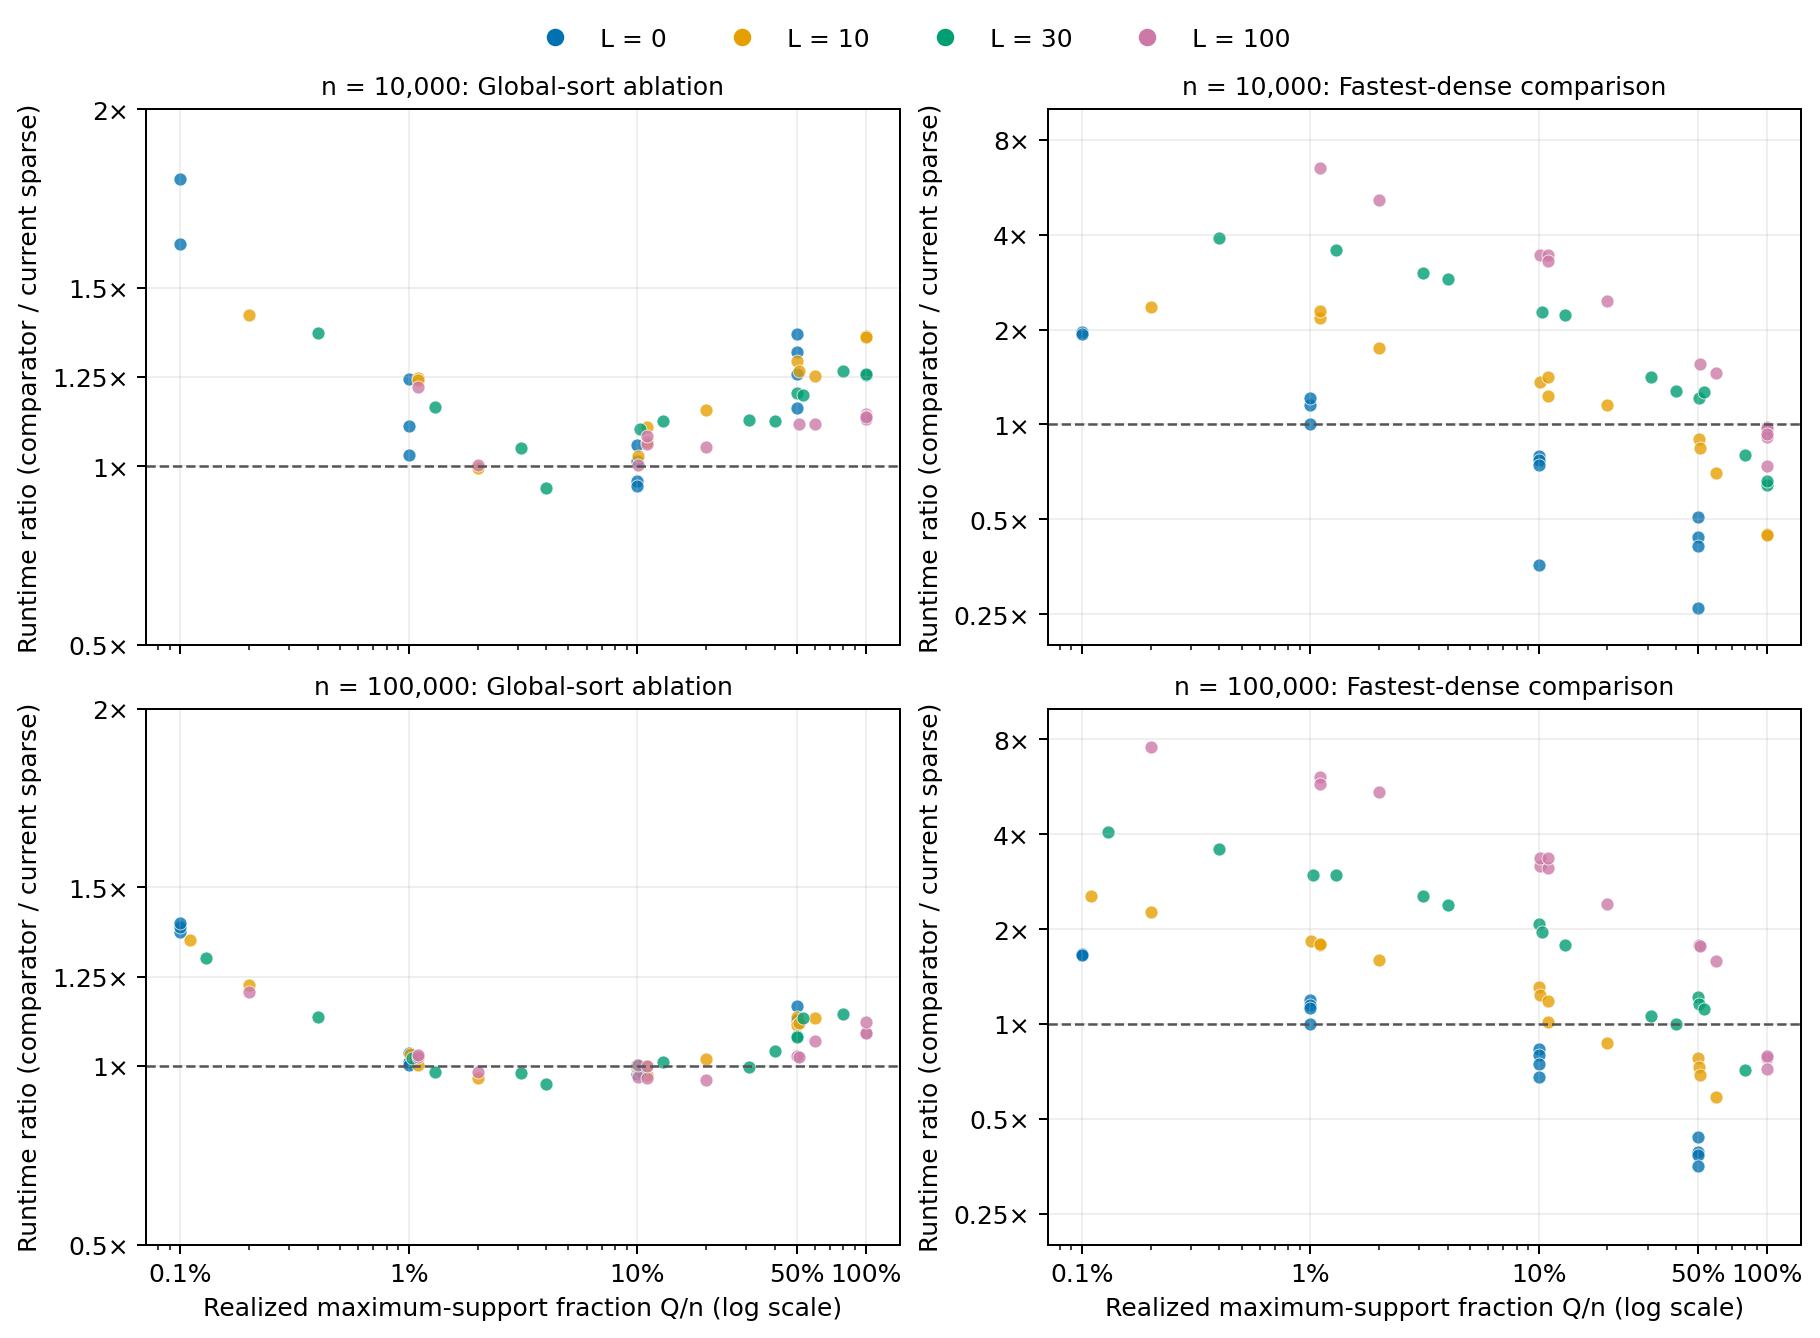
\includegraphics[width=\linewidth]{figures/mechanism.readable.png}
\caption{Mechanism ablation: each point is one predeclared synthetic cell,
using medians of three randomized repetitions. Support fraction $Q/n$ is
measured after expansion. The dense comparator is the fastest of three dense
implementations. The full-sort variant keeps support grouping and the compiled
sparse integration kernel fixed.}
\label{fig:mechanism}
\end{figure}

\subsection{Published implementation across source families}
The post-review supplement selects the shortest and median-length series
within each family, deduplicating coincident choices. It contains
42 full-length series from all 23
families, uses Chronos-Bolt base scores and $L=30$, and preserves all vectors.
Methods run in a seeded random order, with three repetitions per method.
Each call has a ten-second post-warmup time limit; late or unfinished calls
are recorded as right-censored. Compilation and subprocess startup are
excluded. Table~\ref{tab:external} reports speed ratios only for completed
pairs, whose subset differs across threshold modes. No numerical speed ratio
is imputed for a censored result.

\begin{table}[htbp]
\centering
\begin{tabular}{lrrrr}
\toprule
dtaianomaly mode & Completed & Censored & Families represented & Median ratio \\
\midrule
250 thresholds & 42 & 0 & 23 & 8.17$\times$ \\
All thresholds & 35 & 7 & 19 & 143.85$\times$ \\
\bottomrule
\end{tabular}
\caption{Actual pinned dtaianomaly code on 42 source-stratified
full-length inputs. Ratios divide the published baseline's median time by
compiled sparse exact evaluation. The 250-threshold row compares an
approximation with exact computation. Completion-conditioned medians are
not full-corpus runtime estimates. Family counts require at least one completed
pair within the family.}
\label{tab:external}
\end{table}

The maximum absolute discrepancy for returned outputs, compared with the
corresponding exact or 250-threshold main result, is
$9.55\times10^{-15}$. All selection, timeout, environment,
and per-call receipts are retained.


\subsection{Padding sensitivity and effect sizes}
Table~\ref{tab:padding} reports all pairs, including small effects.
All 350 series and 23 source families remain eligible in each variant.
The largest newly computed exact-versus-dense discrepancy is
$2.37\cdot10^{-13}$; 144 transformed small-case upstream checks also pass.
Of 84 original PR reversals, 75 persist after filling and 74 on the suffix,
all in the same direction. Filling removes nine and introduces 18; cropping
removes ten and introduces 21. Thus documented zero padding alone does not
explain the effect, while individual changed orders depend on preprocessing.

\begin{table}[t]
\centering
\begin{tabular}{lrrrr}
\toprule
Variant & PR reversals & Series & Top changes & ROC reversals\\
\midrule
Released & 84 & 55 & 50 & 5\\
First-score fill & 93 & 59 & 52 & 12\\
Common suffix & 95 & 61 & 48 & 8\\
\bottomrule
\end{tabular}
\caption{Each row has 2,100 unordered model-pair comparisons and 700
series/width decisions. A reversal has opposite signs with both gaps
above $10^{-10}$. Top changes require a unique best model in both calculations.}
\label{tab:padding}
\end{table}

Most reversals have small margins. Requiring both exact and sampled PR gaps
to be at least $10^{-3}$ leaves 38, 41, and 44 reversals in the three variants;
at $10^{-2}$ each has five. On the common suffix the median, 95th-percentile,
and maximum absolute PR errors are $0.002489$, $0.177261$, and $0.582639$.
Giving source families equal weight yields reversal prevalences of
2.44\%, 5.45\%, and 4.31\%, with descriptive family-bootstrap intervals
[1.12,4.06]\%, [2.12,10.32]\%, and [1.84,7.59]\%, respectively.
These differ from the pooled pair fractions 4.00\%, 4.43\%, and 4.52\%;
singleton families cannot support precise population estimates.
The result concerns approximation-induced metric order, not a change in
detector quality or a claim that the exact metric is the best model selector.

\section{Error-bounded refinement along the width axis}
\label{sec:width}
Exact threshold integration leaves a second cost: evaluating every integer
width. We next bound the scalar average while omitting selected widths.
This is a different reduction from restricting thresholds. It uses the
geometry of expanded anomaly intervals and a probability-box (p-box)
expectation bound; the latter is established prior work
\cite{utkin2009,troffaes2011}.

\subsection{Where width monotonicity holds}
For consecutive original intervals ending at $e_i$ and starting at $s_{i+1}$,
their expansions first overlap at
\[
 c_i=2\left\lceil\frac{s_{i+1}-e_i}{2}\right\rceil .
\]
The strict overlap convention matters: merely adjacent expansions do not merge.
Partition $0,\ldots,L$ immediately before every distinct $c_i\le L$.
Within each resulting integer interval $[a,b]$, the number $K$ of expanded
segments is constant, each segment expands without merging, and each
threshold's hit count is nondecreasing.

\begin{lemma}[Coordinate order within a merge-free interval]
For a fixed threshold and $a\le w\le b$ in one such interval,
\[
 R_a\le R_w\le R_b,\quad
 \Prec_a\le\Prec_w\le\Prec_b,\quad
 F_a\ge F_w\ge F_b .
\]
At any fixed width, recall and FPR are nondecreasing as the threshold falls.
\end{lemma}
\begin{proof}
Let $O$ be the number of admitted original positives and $B_w$ the admitted
buffer mass. Both $O$ and the prediction count $C$ are fixed across widths,
while $B_w$ is nondecreasing. The unclipped overlap recall is
$(O+B_w)/(P_0+B_w/2)$, whose derivative in $B_w$ is
$(P_0-O/2)/(P_0+B_w/2)^2>0$. Multiplication by the nondecreasing
existence reward $H_w/K$ and clipping preserve order.
Precision is $(O+B_w)/C$. For FPR,
\[
 \frac{\partial F}{\partial B}
 =\frac{-(n-P_0)+(C-O)/2}{(n-P_0-B/2)^2}<0,
\]
since $C-O\le n-P_0$.
Across descending thresholds, original-positive admissions increase $O$;
other admissions increase $B$ and increase the false-positive numerator by
$1-a_i^{(w)}\ge0$ while decreasing its denominator. Thus both curve
coordinates are nondecreasing in threshold order. Ties enter together.
\end{proof}

\begin{theorem}[ROC width enclosure]
Within a merge-free interval, the exact ROC area is nondecreasing in width.
Consequently every omitted width has area in
$[\mathrm{ROC}_a,\mathrm{ROC}_b]$.
\end{theorem}
\begin{proof}
Use the common full threshold sequence, with the prescribed origin and
terminal point. Its trapezoidal area is coordinatewise nondecreasing in each
recall and nonincreasing in each interior FPR:
\[
 \frac{\partial A}{\partial R_j}=\frac{F_{j+1}-F_{j-1}}2\ge0,\qquad
 \frac{\partial A}{\partial F_j}=\frac{R_{j-1}-R_{j+1}}2\le0 .
\]
Linear interpolation between the endpoint coordinate sequences preserves
their threshold monotonicity. Apply the coordinate-order lemma along this
interpolation. Sparse event integration gives the same scalar area.
\end{proof}

Neither global ROC monotonicity nor PR-area monotonicity is assumed.
For example, with $n=20$, positive positions $\{0,2,19\}$ and scores
$(20,4,19,3,18,17,16,15,14,13,12,11,10,9,8,7,6,5,2,1)$,
ROC drops from $0.444444$ at width one to $0.405557$ at width two when
three expanded segments become two.
Even without a merge, scalar endpoint PR values need not enclose the
interior. Take $n=700$, positive positions $100,\ldots,199$ and $600$,
and initially zero scores. Assign score three to positions $100,\ldots,149$,
score one to $150,\ldots,199$ and $600$, and score two to
$0,\ldots,99$, $200,\ldots,549$, and $599$. The first merge occurs at
width 402. Direct evaluation gives PR $0.385206$ at width one,
$0.366313$ at width two, and $0.909134$ at width 400.
Thus the width-two area lies below both endpoint values on $[1,400]$.
The artifact verifies this witness independently.

\subsection{PR bounds without monotone precision}
Index the common descending support events by $j=1,\ldots,G$.
At every width, $q_j=R_j-R_{j-1}\ge0$ and $\sum_jq_j=1$, since the
last support event has recall one. Hence PR is an expectation
$\sum_j q_j\Prec_j$, with cumulative distribution $R_j$.
For $z\in(0,1)$, define the feasible quantile window
\[
 \ell(z)=\min\{j:R_{b,j}\ge z\},\qquad
 u(z)=\min\{j:R_{a,j}\ge z\}.
\]
The coordinate-order lemma implies that the quantile index for any
intermediate width belongs to $[\ell(z),u(z)]$.

\begin{theorem}[PR width enclosure]
Every width in $[a,b]$ has exact PR area between
\begin{align}
 L_{a,b}^{\mathrm{PR}}
 &=\int_0^1\min_{\ell(z)\le j\le u(z)}\Prec_{a,j}\,dz,\\
 U_{a,b}^{\mathrm{PR}}
 &=\int_0^1\max_{\ell(z)\le j\le u(z)}\Prec_{b,j}\,dz .
\end{align}
Both bounds can be computed in $O(G)$ time and space.
\end{theorem}
\begin{proof}
The quantile representation of $\sum_jq_j\Prec_j$ integrates the precision
at the quantile index over $z$. That index lies in the displayed window,
and its precision is between the corresponding endpoint precisions.
Taking the window minimum and maximum and integrating yields the bounds.
Breakpoints are the union of the two endpoint recall sequences. Merge them
in linear time. Both ends of the index window move only right; standard
monotone deques maintain the precision minimum and maximum in amortized
constant work per inserted or removed index. Each index is inserted and
removed at most once.
\end{proof}
These are extrema over a relaxed p-box model, not necessarily values
attained by an intermediate VUS width. This relaxation permits a valid bound
despite oscillating precision. We claim the VUS-specific coordinate order,
merge partition, and adaptive use of these bounds, not the general p-box
expectation construction.

\subsection{Adaptive evaluation and decisions}
Evaluate the endpoints of each merge-free interval. If an active interval
$[a,b]$ has $r=b-a-1$ unevaluated interior widths, add $rL_{a,b}$ and
$rU_{a,b}$ to the lower and upper sums, respectively. Add evaluated scalar
values exactly once, then divide by $L+1$. This encloses the target discrete
average; it does not replace it with a continuous-width integral.

Refine the interval with the largest contribution to uncertainty by
evaluating its midpoint and replacing it by two subintervals.
Stop once both metric intervals have half-width at most $\varepsilon$,
or when every width is evaluated. The returned estimate is the midpoint.
One model outranks another whenever its lower bound exceeds the other's
upper bound; overlapping intervals produce no ordering assertion.

With $m$ distinct evaluated widths, preparation, endpoint calculation,
linear p-box bounds and heap refinement take
$O(n\log(Q+1)+mQ+m\log m)$ time.
A fixed-size endpoint-curve cache retains at most eight curves; evicted
endpoints can be recomputed a constant number of times per refinement.
Space is $O(n+Q+m)$, with no width-by-support matrix.
The artifact records both distinct widths and actual curve evaluations.
The bound is output-sensitive to the requested precision and geometry;
neither $m\ll L$ nor a wall-clock improvement is guaranteed.

The theorems are real-arithmetic statements. The implementation uses
float64, clips ulp-scale recall drift, and adds an empirical $10^{-12}$
guard to adaptive endpoints. It is not a directed-rounding interval library.
Experiments independently audit enclosure within $10^{-10}$ and use a
$2\cdot10^{-10}$ separation margin for numerical ordering checks.
These allowances are reported separately from the requested approximation
half-width. Setting $\varepsilon=0$ evaluates every width.

% Measured source: artifacts/advancement/analysis/analysis.json
% SHA-256: 3727de01958ef96deb0c15ad22823506eb9097e975f046334d84976a10e37762
\subsection{Error bounds and the cost of width refinement}
The width-refinement experiment retains the metadata-selected 42 series
covering all 23 families and all three released score vectors. Maximum widths
30, 100, and 300 give 378 model/width cases; the width-300 setting is an
explicit stress condition. Both $\varepsilon=0.01$ and $0.001$ bound the
half-widths of both returned metric intervals. The M1 Pro timing protocol
again includes whole-call preprocessing and uses three randomized-order
repetitions. Table~\ref{tab:width-refinement} compares against full-width
Sparse VUS on these same inputs.

\begin{table}[t]
\centering
\begin{tabular}{rrrrrr}
\toprule
$\varepsilon$ & $L$ & \shortstack{Median\\ratio} & Faster / 126 & \shortstack{Distinct\\widths (\%)} & \shortstack{Curve calls\\(\%)}\\
\midrule
0.01 & 30 & 0.835 & 27 & 16.1 & 16.1 \\
0.01 & 100 & 0.905 & 46 & 7.9 & 7.9 \\
0.01 & 300 & 1.313 & 100 & 4.7 & 7.3 \\
0.001 & 30 & 0.615 & 4 & 54.8 & 80.6 \\
0.001 & 100 & 0.426 & 11 & 39.6 & 74.3 \\
0.001 & 300 & 0.391 & 25 & 25.4 & 53.8 \\
\bottomrule
\end{tabular}
\caption{Full-width exact runtime divided by adaptive runtime. Width and
curve-call columns are medians relative to $L+1$; cache eviction can make
curve calls exceed the number of distinct widths. Values below one indicate
that adaptive evaluation is slower.}
\label{tab:width-refinement}
\end{table}

All 378 cases at both tolerances contain the full-width ROC and PR values
within the separately declared $10^{-10}$ numerical audit allowance.
Maximum midpoint errors are $0.003260$ and $0.000713$ for tolerances 0.01
and 0.001. However, fewer width evaluations do not generally imply faster
execution. Across all three maximum widths, median runtime ratios are
0.966 and 0.467, with adaptive evaluation faster in 173 and 40 of 378 cases,
respectively. At tolerance 0.01 and $L=300$, the geometric mean ratio is
1.370 (series-bootstrap interval [1.207,1.557]); at the tighter tolerance,
all three width groups have geometric mean ratios below one.
The present implementation therefore provides useful enclosures, but the
standalone fixed-tolerance strategy is often slower than exact evaluation.

As a numerical decision replay, nonoverlapping PR intervals identify unique
winners in 21, 17, and 15 of the 42 series at tolerance 0.01 for widths
30, 100, and 300; the corresponding counts at tolerance 0.001 are 33, 32,
and 34. All asserted winners agree with exact PR using the declared
$2\cdot10^{-10}$ separation margin. These replay counts do not include
additional decision-workload timing or establish a model-selection speedup.

Separately authored validation directly constructs full-threshold curves
for every both-class binary label vector of lengths two through seven,
using four seeded score patterns per vector. It checks 13,776 widths and
width enclosures and 960 discrete averages. The largest curve discrepancy
is $6.67\cdot10^{-16}$ and the largest enclosure violation is
$3.34\cdot10^{-16}$, within the declared $2\cdot10^{-12}$ allowance.
A further 760 linear-programming comparisons of p-box extrema have maximum
discrepancy $3.34\cdot10^{-16}$. Exhaustiveness concerns labels only, not all
rankings or tie patterns; these checks audit the implementation and complement
the real-arithmetic proofs.



\section{Incremental PR model selection}
\label{sec:racing}
Fixed-tolerance evaluation asks each model to meet an absolute error target
before using the resulting intervals to select a winner. This can over-refine
already separable models and repeat preparation during exact fallback.
We therefore also study an incremental PR race. It was designed after
inspecting the standalone fixed-tolerance width-refinement results;
its measurements are a separate
post-hoc follow-up on the same 126 series/width selection tasks.

For each of $M$ models, prepare its sparse evaluator once and initialize
the endpoints of every merge-free width block. Retain all observed PR scalars,
an endpoint-curve cache, and a heap of unevaluated interiors. An interior
$(a,b)$ has priority $(b-a-1)(U_{a,b}^{\mathrm{PR}}-L_{a,b}^{\mathrm{PR}})$.
Its midpoint refinement reuses preparation and updates the model's global
PR enclosure $[\ell_k,u_k]$. The reused endpoint oracle still computes ROC,
but only PR ordering controls selection; there is no predetermined
scalar-error target.

After initialization and every refinement, rescreen \emph{all} models.
Return a singleton $k$ only if
$\ell_k>u_j+\eta$ for every $j\ne k$, where $\eta=3\cdot10^{-10}$.
Otherwise the current candidate set is
\[
 \mathcal C=\{k:u_k\ge\max_j\ell_j-\eta\}.
\]
This is repeated screening, not permanent deletion; a model outside
$\mathcal C$ retains its state and is checked again.
Among nonexact candidates, refine the model with the widest global PR interval,
breaking ties by model name, and bisect its highest-priority width interior.
If all candidates are exact, return every candidate whose exact PR is within
$\tau=10^{-10}$ of their maximum. Exact means use already observed widths;
no second preparation or separate exact evaluator is called.
The no-pruning ablation keeps all models in $\mathcal C$ whenever the
singleton condition fails, retaining the same stopping and refinement rules.

\begin{proposition}[Finite decision resolution]
With valid real-arithmetic width enclosures and $\eta>\tau$, the race returns
the exact $\tau$-tie set and evaluates at most $M(L+1)$ distinct model/width
pairs.
\end{proposition}
\begin{proof}
A separated winner exceeds every other true PR by more than $\eta$.
A currently excluded model has true PR more than $\eta$ below some model's
lower bound, hence cannot belong to the global $\tau$-tie set.
At least one candidate exists. Each refinement evaluates one unseen width
in a nonempty interior; active interiors are disjoint. Therefore at most
$M(L+1)$ distinct pairs can be observed. If separation does not occur, all
remaining candidates eventually become exact and the tie rule resolves them.
\end{proof}

Let $T$ be the number of refinements and $m_k$ the number of distinct widths
queried for model $k$. In addition to one preparation per model, endpoint work
is $O(Q\sum_km_k)$, heap work is $O(T\log(L+1))$, and rescreening is $O(MT)$.
With the default cache, actual curve calls are at most the initialization
count plus $3T$; both actual calls and distinct widths are recorded.
Close scores can require full evaluation, and decision bookkeeping can
outweigh avoided curves. The float64 implementation retains the empirical
$10^{-12}$ guard; the ordering margin is a numerical allowance, not a
directed-rounding proof.

\IfFileExists{selection_results.tex}{% Generated by experiments/analyze_selection.py
% Analysis SHA-256: c985a62b74087d99f60a7afc440a369df272c34a5255b9f5905b3e3f5cf67c31
\subsection{Complete model-selection workloads}
We select the maximum exact PR among all three released score vectors,
retaining every model within $10^{-10}$ of the maximum.
Both experiments use the same fixed 42-series metadata selection and
$L\in\{30,100,300\}$ (126 tasks), with no case exclusions.
Every timed call includes all model preparation and all subsequent
refinement or fallback; score loading and warmed JIT compilation are
excluded. Model training and inference are not measured.
Width 300 remains an explicit stress regime.
\paragraph{Fixed tolerance with exact fallback.}
At initial half-width $0.01$, the selector's median speed ratios
against sparse exact selection are
$0.579\times$, $0.569\times$, and $0.738\times$.
All 126 decisions agree, but the complete selector is slower at every
width in the median. Pruning reduces exact fallback model evaluations
from 63/75/81 to 53/63/69, without recovering this overhead.
The fixed-250 comparator changes the selected set in 4/5/5 tasks.
Of these, 3/4/4 have a unique exact winner; the remaining
case at each width breaks an exact three-way tie.
\paragraph{Incremental PR racing.}
The follow-up removes the fixed accuracy target and reuses each model's
prepared state (Section~\ref{sec:racing}). This design was chosen after
observing the fixed-tolerance overhead; it is not a preregistered
independent generalization study. Fresh timings on both architectures
retain the same inputs and separate each executable exact comparator.
Every racing decision agrees with exact selection on both platforms.
\begin{table}[t]\centering
\begin{tabular}{llrrrrrr}\toprule
Platform & $L$ & vs.\ sparse & vs.\ oracle & wins/42 & exact ms & race ms & widths \\\midrule
macOS & 30 & 0.829 & 0.829 & 8 & 9.08 & 12.96 & 18.3\% \\
macOS & 100 & 0.715 & 0.678 & 11 & 16.57 & 23.72 & 16.3\% \\
macOS & 300 & 1.177 & 1.063 & 22 & 38.34 & 41.37 & 10.5\% \\
Linux & 30 & 0.817 & 0.796 & 8 & 9.11 & 13.93 & 18.3\% \\
Linux & 100 & 0.757 & 0.704 & 10 & 18.90 & 27.04 & 16.3\% \\
Linux & 300 & 1.376 & 1.216 & 26 & 49.06 & 45.16 & 10.5\% \\
\bottomrule\end{tabular}
\caption{Incremental PR selection, 42 tasks per row. Ratios above one
favor racing. The oracle chooses the fastest of three separately
measured compiled exact methods per task; it is not deployable.
Wins compare racing to that oracle; latency columns are medians in
milliseconds for sparse exact and racing. Widths is the median fraction
of the $3(L+1)$ distinct model-width queries evaluated. Recomputed
endpoint curves are separately counted in the released records.}
\label{tab:selection}\end{table}
\paragraph{Median gain versus total cost.}
At width 300 on macOS, summing the 42 case medians gives 10.615\,s for racing versus 6.249\,s for sparse exact evaluation (more total time).
At width 300 on Linux, summing the 42 case medians gives 10.522\,s for racing versus 7.051\,s for sparse exact evaluation (more total time).
Thus the distribution median and the total workload cost must be read separately; a positive median speed ratio does not establish net time savings.
The no-pruning ablation retains the separated-winner rule and refines
all models when no winner separates. Its median time divided by the
pruning variant's time, at the three increasing widths, is
macOS: $1.022$, $1.032$, $1.094$;
Linux: $1.018$, $1.056$, $1.088$;
these values isolate the incremental effect of pruning in this workload.
All bound-separation decisions are numerical audits under the stated
$10^{-10}$ enclosure allowance, not formal Float64 certificates.
The artifact includes absolute totals, series-clustered intervals,
full-evaluation counts, and every slower task.
}{}
\subsection{PR-only execution with a bounded endpoint budget}
\label{sec:pr-engine}
The negative aggregate-cost result for the preceding racer motivated a
disclosed implementation follow-up. The earlier engine crosses Python and
NumPy boundaries during refinement, constructs ROC coordinates even for PR
selection, and can recompute evicted endpoint curves. Saving distinct width
queries therefore need not save actual curve calculations or time.

The follow-up executes the controller and PR curve calculations in compiled
code. A single quantile traversal maintains separate minimum and maximum
deques to compute both p-box extrema, avoiding materialized breakpoint and
coordinate-envelope arrays. It computes the same real-arithmetic bounds;
this is an execution change, not a new p-box theorem. Each observed width's
scalar is retained. Endpoint coordinates are never evicted during adaptive
refinement: before their budget is exhausted, that model switches to an
exhaustive sweep of only its unobserved widths, reusing preparation and
scratch storage. No public exact-evaluator call restarts the computation.

Let $W=L+1$, $G_m$ be model $m$'s number of distinct support-score groups,
and $Q$ be the maximum-support size. The endpoint capacity is
\[
 C_m=\min\!\left(W,\max(2,\lfloor\alpha W\rfloor),
             \left\lfloor\frac{B}{16G_m}\right\rfloor\right),
\]
with $C_m=0$ when $\alpha=0$. If a model's initial merge-block endpoints
already exceed this capacity, it uses exact completion immediately. The
declared initial policy uses $\alpha=1/8$ and $B=8$ MiB per model. Two
Float64 coordinate arrays per retained endpoint account for the factor 16;
$B$ does not bound process RSS or all auxiliary memory.

Each model performs at most $W$ actual width evaluations, including exact
completion, because an observed scalar is never evaluated again. The
artifact separately counts adaptive and completion evaluations. In addition
to prepared inputs, retained coordinates use at most $\sum_m16C_mG_m$
bytes, with $O(MW)$ scalar and controller state. The implementation scans
the model-by-width state when updating global bounds and scans interval
priorities during refinement. Including the initial state scans, its bookkeeping
can require $O(MW(1+\sum_m C_m))$ work, bounded above by $O(M^2W^2)$ when capacity scales
with width. Consequently the endpoint budget is a query/storage guarantee,
not a constant-factor wall-clock overhead guarantee.

An equally specialized exhaustive PR-only sparse kernel and an independent
PR-only dense kernel are required controls. The former uses the same
unobserved-width completion primitive with every width initially unknown;
the latter constructs the sum-and-clip ramps directly. Both execute all
widths in one compiled call and reuse scratch arrays. Thus any advantage of
the new racer must survive comparison with an exact method that also omits
ROC work. Before the policy holdout, two further parameter-free controls
receive the same global radix ranking: one retains direct ramp construction,
and one uses the same linear nearest-interval geometry and weight formula
as the sparse method. Both still traverse every input position and complete
every numerical tie at every width, computing PR alone. These controls
separate generic radix and geometry gains from sparse event elimination;
the nearest variant takes $O((L+1)n)$ time and $O(n+K)$ auxiliary memory.
Float64 guards, separation margins and exact-tie conventions are
unchanged. This follow-up does not replace the earlier negative results.


\begin{thebibliography}{99}
\bibitem{paparrizos2022} J. Paparrizos et al. Volume Under the Surface: A New Accuracy Evaluation Measure for Time-Series Anomaly Detection. PVLDB 15(11), 2022. \url{https://www.vldb.org/pvldb/vol15/p2774-paparrizos.pdf}.
\bibitem{boniol2025} P. Boniol et al. VUS: Effective and Efficient Accuracy Measures for Time-Series Anomaly Detection. VLDB Journal 34, 2025. \url{https://arxiv.org/abs/2502.13318}.
\bibitem{sylligardos2025} E. Sylligardos. Fast or Accurate? Rethinking Time Series Anomaly Detection. VLDB PhD Workshop, 2025, Section 4. \url{https://www.vldb.org/2025/Workshops/VLDB-Workshops-2025/PhD/PhD25_17.pdf}.
\bibitem{boxer} P. Stergiotis. boxer/adscore, v0.0.23, 2026. \url{https://pkg.go.dev/github.com/stergiotis/boxer/public/analytics/timeseries/adscore}.
\bibitem{dtaianomaly} ML-KULeuven. dtaianomaly, pinned revision \texttt{557b4357}, 13 October 2026. \url{https://github.com/ML-KULeuven/dtaianomaly}.
\bibitem{klein2026} T. L. Klein. fast-VUS. Software repository, first commit 12 October 2026, audited revision \texttt{1bae859f}, 16 October 2026. \url{https://github.com/tomlouisklein/fast-VUS}.
\bibitem{ffvus2026} E. Sylligardos. FF-VUS implementation in aVUSi. Software, audited revision \texttt{facf4362}, 23 June 2026. \url{https://github.com/doanthihoaithu/aVUSi}.
\bibitem{benchopt2026} Benchopt contributors. Time-series foundation-model benchmark: VUS metrics. Software, audited revision \texttt{2b55ccb1}, 29 September 2026. \url{https://github.com/benchopt/benchmark_tsfm}.
\bibitem{herf2001radix} M. Herf. \emph{Radix Tricks}. December 2001. \url{https://stereopsis.com/radix.html}. Accessed 2026-10-21.
\bibitem{demaine2011radix} E. Demaine. \emph{Lecture 7: Linear-Time Sorting}. MIT OpenCourseWare, 6.006 Introduction to Algorithms, Fall 2011. \url{https://ocw.mit.edu/courses/6-006-introduction-to-algorithms-fall-2011/bf7d79105762bf79bbc0925438e1468a_MIT6_006F11_lec07.pdf}. Accessed 2026-10-21.
\bibitem{utkin2009} L. Utkin and S. Destercke. Computing Expectations with Continuous P-Boxes: Univariate Case. International Journal of Approximate Reasoning 50(5), 778--798, 2009. \url{https://doi.org/10.1016/j.ijar.2009.02.004}.
\bibitem{troffaes2011} M. C. M. Troffaes and S. Destercke. Probability Boxes on Totally Preordered Spaces for Multivariate Modelling. International Journal of Approximate Reasoning 52, 767--791, 2011. \url{https://doi.org/10.1016/j.ijar.2011.02.001}.
\bibitem{zhu2026} X. Zhu, L. Carpentier, M. Verbeke. When Foundation Models are One-Liners: Limitations and Future Directions for Time Series Anomaly Detection. ICLR 2026. Scores: KU Leuven RDR, V1, \url{https://doi.org/10.48804/MCVI4N}.
\bibitem{tsbad} Q. Liu and J. Paparrizos. The Elephant in the Room: Towards a Reliable Time-Series Anomaly Detection Benchmark. NeurIPS Datasets and Benchmarks, 2024. \url{https://github.com/TheDatumOrg/TSB-AD}.
\bibitem{esa2024} K. Kotowski et al. European Space Agency Benchmark for Anomaly Detection in Satellite Telemetry. 2024, revised 2025. \url{https://arxiv.org/abs/2406.17826}.
\end{thebibliography}
% END SHARED BODY
\end{document}
